% Options for packages loaded elsewhere
\PassOptionsToPackage{unicode}{hyperref}
\PassOptionsToPackage{hyphens}{url}
%
\documentclass[
  ignorenonframetext,
]{beamer}
\usepackage{pgfpages}
\setbeamertemplate{caption}[numbered]
\setbeamertemplate{caption label separator}{: }
\setbeamercolor{caption name}{fg=normal text.fg}
\beamertemplatenavigationsymbolsempty
% Prevent slide breaks in the middle of a paragraph
\widowpenalties 1 10000
\raggedbottom
\setbeamertemplate{part page}{
  \centering
  \begin{beamercolorbox}[sep=16pt,center]{part title}
    \usebeamerfont{part title}\insertpart\par
  \end{beamercolorbox}
}
\setbeamertemplate{section page}{
  \centering
  \begin{beamercolorbox}[sep=12pt,center]{part title}
    \usebeamerfont{section title}\insertsection\par
  \end{beamercolorbox}
}
\setbeamertemplate{subsection page}{
  \centering
  \begin{beamercolorbox}[sep=8pt,center]{part title}
    \usebeamerfont{subsection title}\insertsubsection\par
  \end{beamercolorbox}
}
\AtBeginPart{
  \frame{\partpage}
}
\AtBeginSection{
  \ifbibliography
  \else
    \frame{\sectionpage}
  \fi
}
\AtBeginSubsection{
  \frame{\subsectionpage}
}
\usepackage{amsmath,amssymb}
\usepackage{lmodern}
\usepackage{iftex}
\ifPDFTeX
  \usepackage[T1]{fontenc}
  \usepackage[utf8]{inputenc}
  \usepackage{textcomp} % provide euro and other symbols
\else % if luatex or xetex
  \usepackage{unicode-math}
  \defaultfontfeatures{Scale=MatchLowercase}
  \defaultfontfeatures[\rmfamily]{Ligatures=TeX,Scale=1}
\fi
\usetheme[]{Singapore}
\usefonttheme{serif}
% Use upquote if available, for straight quotes in verbatim environments
\IfFileExists{upquote.sty}{\usepackage{upquote}}{}
\IfFileExists{microtype.sty}{% use microtype if available
  \usepackage[]{microtype}
  \UseMicrotypeSet[protrusion]{basicmath} % disable protrusion for tt fonts
}{}
\makeatletter
\@ifundefined{KOMAClassName}{% if non-KOMA class
  \IfFileExists{parskip.sty}{%
    \usepackage{parskip}
  }{% else
    \setlength{\parindent}{0pt}
    \setlength{\parskip}{6pt plus 2pt minus 1pt}}
}{% if KOMA class
  \KOMAoptions{parskip=half}}
\makeatother
\usepackage{xcolor}
\IfFileExists{xurl.sty}{\usepackage{xurl}}{} % add URL line breaks if available
\IfFileExists{bookmark.sty}{\usepackage{bookmark}}{\usepackage{hyperref}}
\hypersetup{
  pdftitle={Bayesian Statistics with R-INLA},
  pdfauthor={Instructor: Sara Martino},
  hidelinks,
  pdfcreator={LaTeX via pandoc}}
\urlstyle{same} % disable monospaced font for URLs
\newif\ifbibliography
\usepackage{color}
\usepackage{fancyvrb}
\newcommand{\VerbBar}{|}
\newcommand{\VERB}{\Verb[commandchars=\\\{\}]}
\DefineVerbatimEnvironment{Highlighting}{Verbatim}{commandchars=\\\{\}}
% Add ',fontsize=\small' for more characters per line
\usepackage{framed}
\definecolor{shadecolor}{RGB}{248,248,248}
\newenvironment{Shaded}{\begin{snugshade}}{\end{snugshade}}
\newcommand{\AlertTok}[1]{\textcolor[rgb]{0.94,0.16,0.16}{#1}}
\newcommand{\AnnotationTok}[1]{\textcolor[rgb]{0.56,0.35,0.01}{\textbf{\textit{#1}}}}
\newcommand{\AttributeTok}[1]{\textcolor[rgb]{0.77,0.63,0.00}{#1}}
\newcommand{\BaseNTok}[1]{\textcolor[rgb]{0.00,0.00,0.81}{#1}}
\newcommand{\BuiltInTok}[1]{#1}
\newcommand{\CharTok}[1]{\textcolor[rgb]{0.31,0.60,0.02}{#1}}
\newcommand{\CommentTok}[1]{\textcolor[rgb]{0.56,0.35,0.01}{\textit{#1}}}
\newcommand{\CommentVarTok}[1]{\textcolor[rgb]{0.56,0.35,0.01}{\textbf{\textit{#1}}}}
\newcommand{\ConstantTok}[1]{\textcolor[rgb]{0.00,0.00,0.00}{#1}}
\newcommand{\ControlFlowTok}[1]{\textcolor[rgb]{0.13,0.29,0.53}{\textbf{#1}}}
\newcommand{\DataTypeTok}[1]{\textcolor[rgb]{0.13,0.29,0.53}{#1}}
\newcommand{\DecValTok}[1]{\textcolor[rgb]{0.00,0.00,0.81}{#1}}
\newcommand{\DocumentationTok}[1]{\textcolor[rgb]{0.56,0.35,0.01}{\textbf{\textit{#1}}}}
\newcommand{\ErrorTok}[1]{\textcolor[rgb]{0.64,0.00,0.00}{\textbf{#1}}}
\newcommand{\ExtensionTok}[1]{#1}
\newcommand{\FloatTok}[1]{\textcolor[rgb]{0.00,0.00,0.81}{#1}}
\newcommand{\FunctionTok}[1]{\textcolor[rgb]{0.00,0.00,0.00}{#1}}
\newcommand{\ImportTok}[1]{#1}
\newcommand{\InformationTok}[1]{\textcolor[rgb]{0.56,0.35,0.01}{\textbf{\textit{#1}}}}
\newcommand{\KeywordTok}[1]{\textcolor[rgb]{0.13,0.29,0.53}{\textbf{#1}}}
\newcommand{\NormalTok}[1]{#1}
\newcommand{\OperatorTok}[1]{\textcolor[rgb]{0.81,0.36,0.00}{\textbf{#1}}}
\newcommand{\OtherTok}[1]{\textcolor[rgb]{0.56,0.35,0.01}{#1}}
\newcommand{\PreprocessorTok}[1]{\textcolor[rgb]{0.56,0.35,0.01}{\textit{#1}}}
\newcommand{\RegionMarkerTok}[1]{#1}
\newcommand{\SpecialCharTok}[1]{\textcolor[rgb]{0.00,0.00,0.00}{#1}}
\newcommand{\SpecialStringTok}[1]{\textcolor[rgb]{0.31,0.60,0.02}{#1}}
\newcommand{\StringTok}[1]{\textcolor[rgb]{0.31,0.60,0.02}{#1}}
\newcommand{\VariableTok}[1]{\textcolor[rgb]{0.00,0.00,0.00}{#1}}
\newcommand{\VerbatimStringTok}[1]{\textcolor[rgb]{0.31,0.60,0.02}{#1}}
\newcommand{\WarningTok}[1]{\textcolor[rgb]{0.56,0.35,0.01}{\textbf{\textit{#1}}}}
\usepackage{longtable,booktabs,array}
\usepackage{calc} % for calculating minipage widths
\usepackage{caption}
% Make caption package work with longtable
\makeatletter
\def\fnum@table{\tablename~\thetable}
\makeatother
\setlength{\emergencystretch}{3em} % prevent overfull lines
\providecommand{\tightlist}{%
  \setlength{\itemsep}{0pt}\setlength{\parskip}{0pt}}
\setcounter{secnumdepth}{-\maxdimen} % remove section numbering
% handouts
\usepackage{handoutWithNotes} 
% put 3 slides on 1 page with space for notes
%\pgfpagesuselayout{3 on 1 with notes}[a4paper, border shrink=5mm]

\setbeamertemplate{navigation symbols}{}
\setbeamertemplate{footline}[page number]

% smaller space in between lines in toc
\makeatletter
\patchcmd{\beamer@sectionintoc}{\vskip1.5em}{\vskip0.5em}{}{}
\makeatother


% two columns environmnt
\newenvironment{cols}[1][]{}{}

\newenvironment{col}[1]{\begin{minipage}{#1}\ignorespaces}{%
\end{minipage}
\ifhmode\unskip\fi
\aftergroup\useignorespacesandallpars}

\def\useignorespacesandallpars#1\ignorespaces\fi{%
#1\fi\ignorespacesandallpars}

\makeatletter
\def\ignorespacesandallpars{%
  \@ifnextchar\par
    {\expandafter\ignorespacesandallpars\@gobble}%
    {}%
}
\makeatother

%% logo on first page
\titlegraphic{\centering 
\includegraphics[width=6cm]{log_ntnu.jpg}}
\ifLuaTeX
  \usepackage{selnolig}  % disable illegal ligatures
\fi

\title{Bayesian Statistics with R-INLA}
\subtitle{University of Zurich, March, 2022}
\author{Instructor: Sara Martino}
\date{}

\begin{document}
\frame{\titlepage}

\begin{frame}[allowframebreaks]
  \tableofcontents[hideallsubsections]
\end{frame}
\begin{frame}
\end{frame}

\begin{frame}{Plan for this 2-day course}
\protect\hypertarget{plan-for-this-2-day-course}{}
\textbf{Today}

\begin{itemize}
\tightlist
\item
  \textbf{9:00-10:45}Introduction and basics concepts of INLA
\item
  \textbf{11:00-12:30} Practical session I
\end{itemize}

\textbf{\textcolor{red}{Lunch}}

\begin{itemize}
\tightlist
\item
  \textbf{13:30-15:00} R-INLA: Basics
\item
  \textbf{15:15-17:00} Practical session II
\end{itemize}
\end{frame}

\begin{frame}[fragile]{Plan for this 2-day course}
\protect\hypertarget{plan-for-this-2-day-course-1}{}
\textbf{Tomorrow}

\begin{itemize}
\tightlist
\item
  \textbf{9:00-10:45} Space time models with \texttt{inlabru}
\item
  \textbf{11:00-12:30} Practical session III
\end{itemize}

\textbf{\textcolor{red}{Lunch}}

\begin{itemize}
\tightlist
\item
  \textbf{13:30-15:00} Advanced topic
\item
  \textbf{15:15-16:00} Practical session IV
\end{itemize}
\end{frame}

\begin{frame}{}
\protect\hypertarget{section}{}
\begin{cols}

\begin{col}{0.5\textwidth}

\begin{center}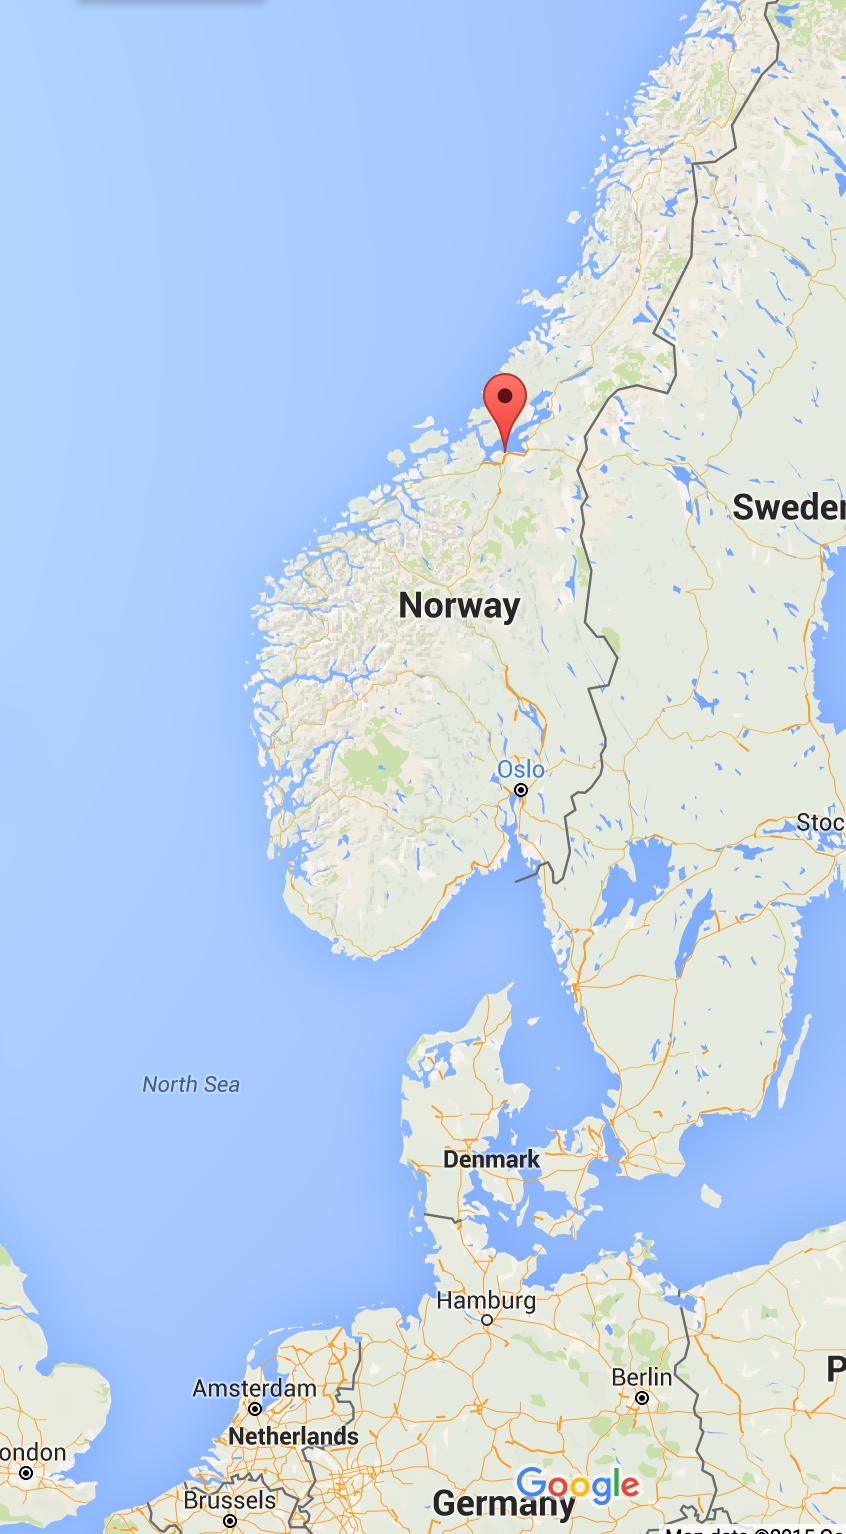
\includegraphics[width=0.95\linewidth]{graphics/tronheimMap} \end{center}

\end{col}

\begin{col}{0.5\textwidth}

\tiny

\begin{center}\includegraphics[width=1.1\linewidth]{graphics/trondheim} \end{center}

\begin{center}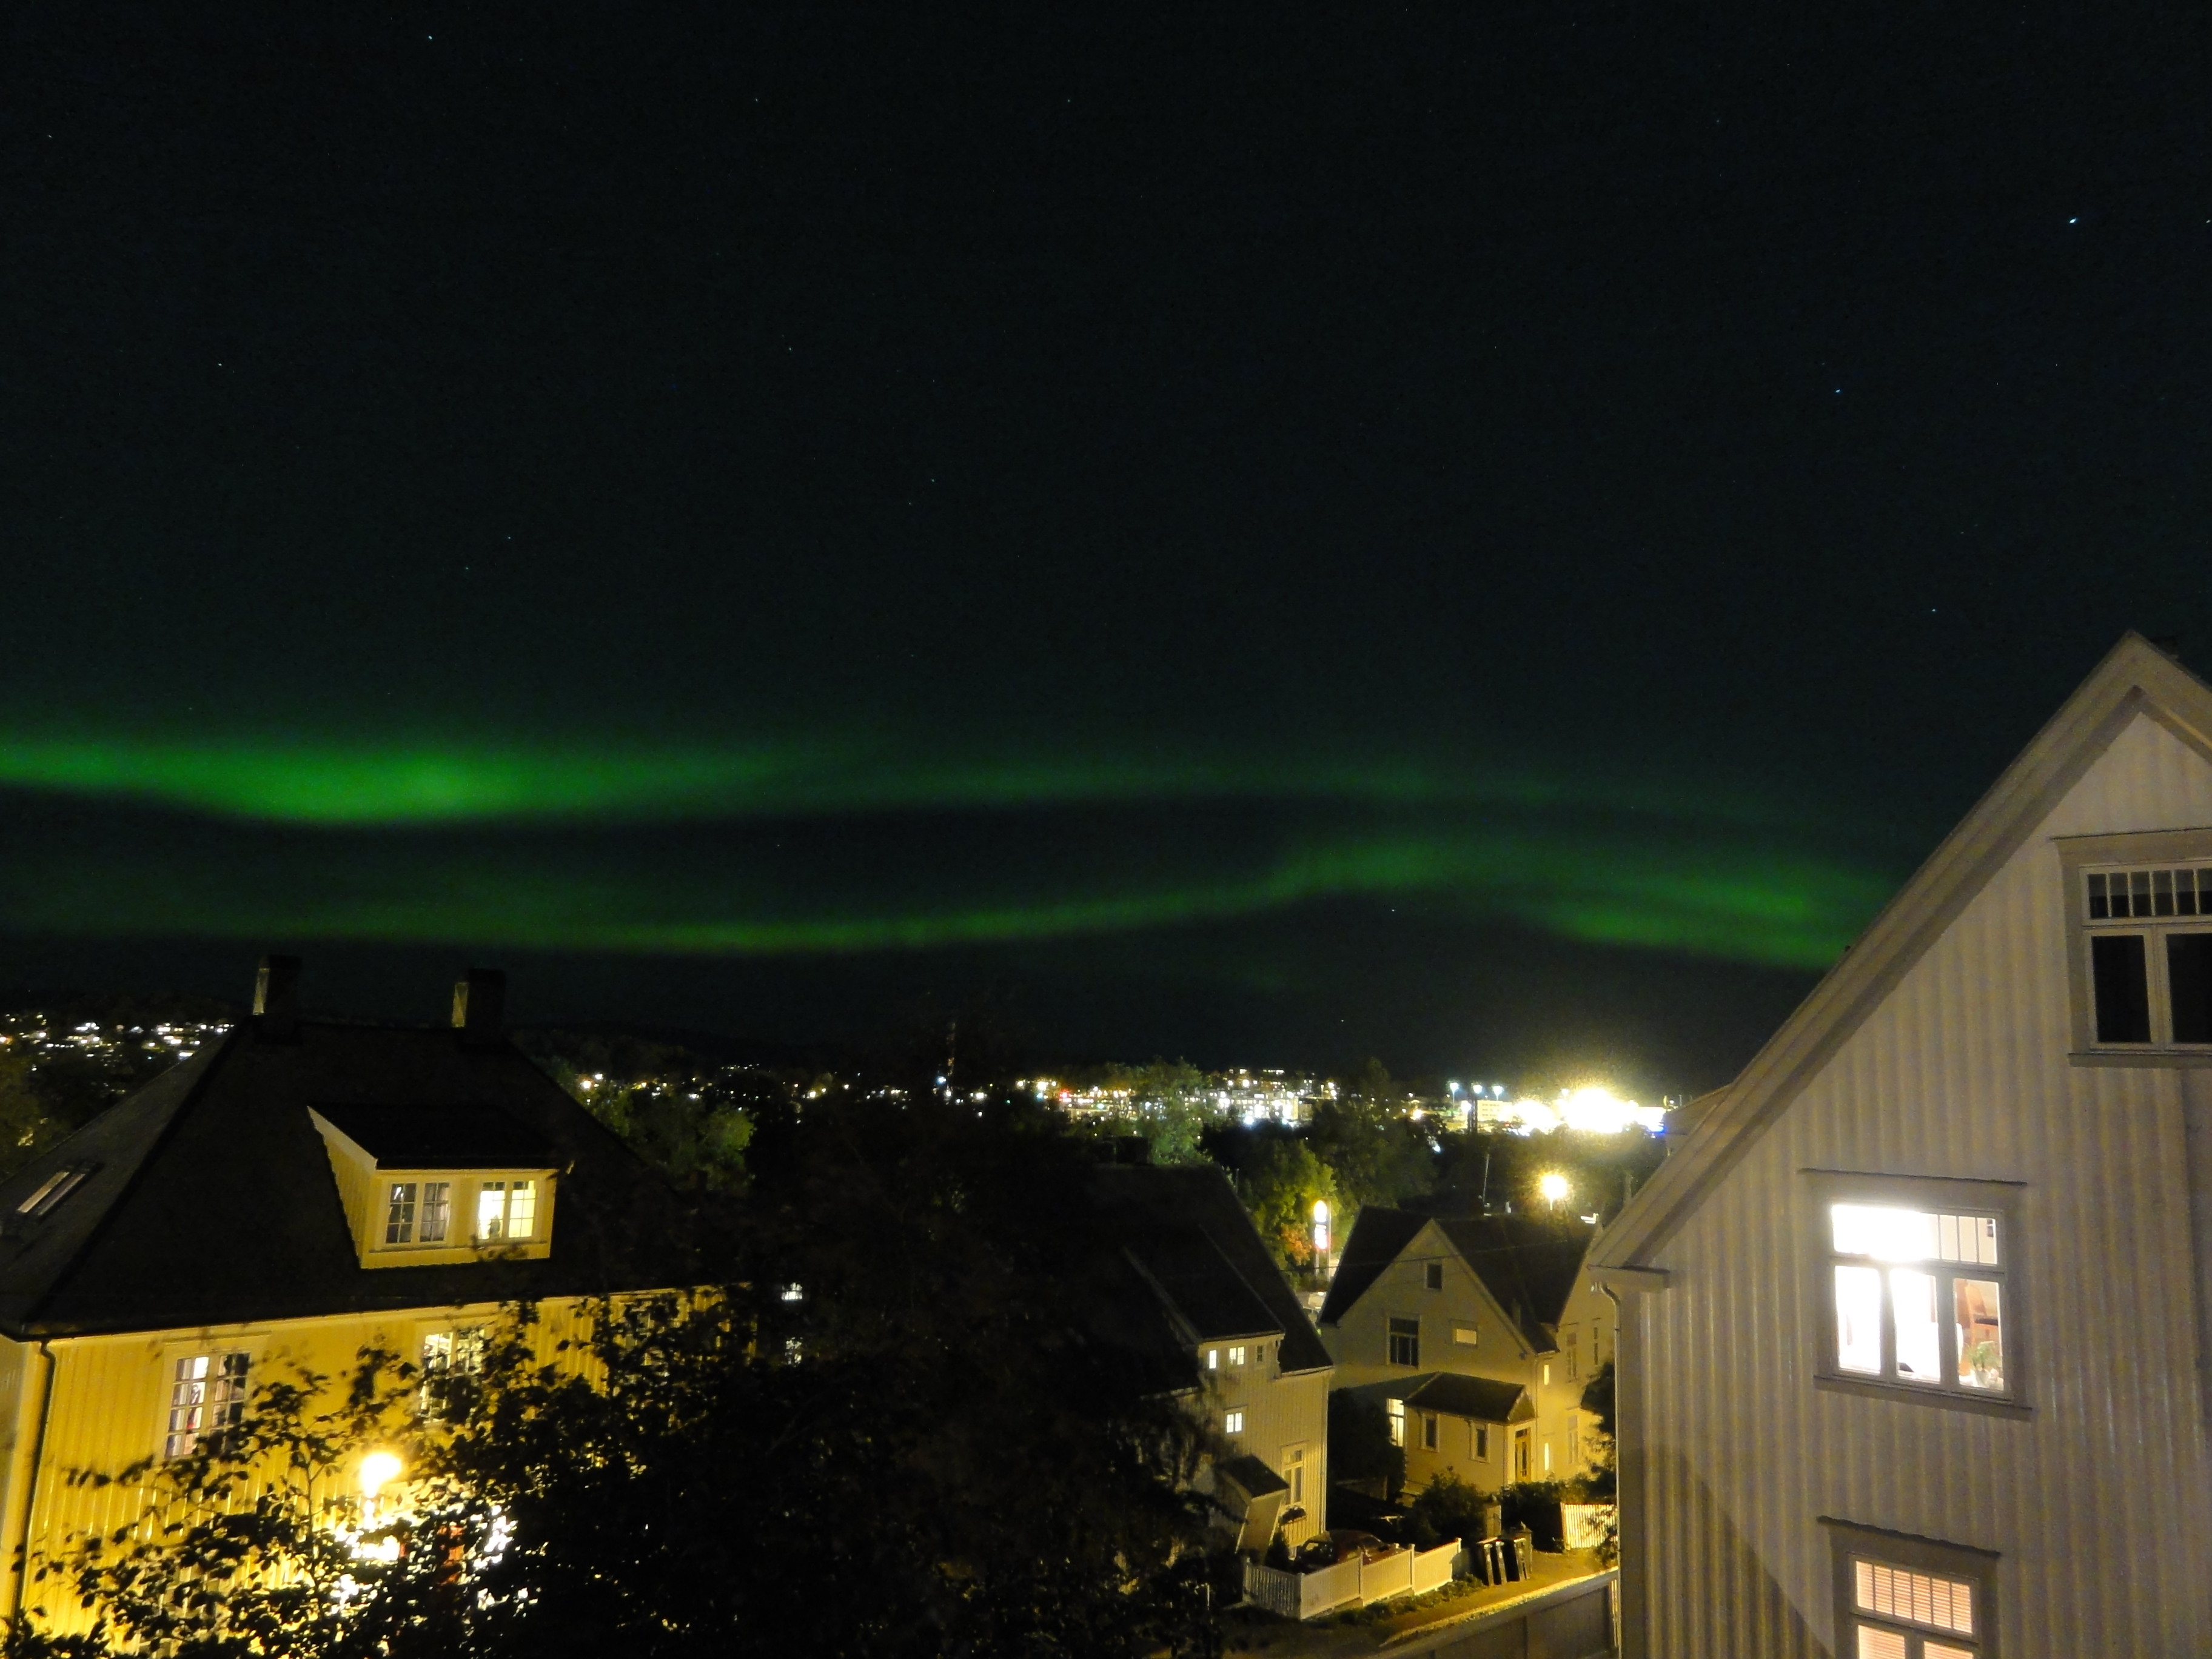
\includegraphics[width=1.1\linewidth]{graphics/nordlys3} \end{center}
\normalsize

\end{col}

\end{cols}
\end{frame}

\hypertarget{introduction}{%
\section{Introduction}\label{introduction}}

\begin{frame}[fragile]{What is inla?}
\protect\hypertarget{what-is-inla}{}
\textbf{The short answer:}\\
\strut \\

\begin{quote}
INLA is a fast method to do Bayesian inference with latent Gaussian
models and \texttt{INLA} is an \texttt{R}-package that implements this
method with a flexible and simple interface.
\end{quote}

\pause

\textbf{The (much) longer answer:}

\begin{itemize}
\tightlist
\item
  Rue, Martino, and Chopin (2009) ``Approximate Bayesian inference for
  latent Gaussian models by using integrated nested Laplace
  approximations.'' \emph{JRSSB}
\item
  Rue, Riebler, Sørbye, Illian, Simpson, Lindgren (2017) ``Bayesian
  Computing with INLA: A Review.'' \emph{Annual Review of Statistics and
  Its Application}
\item
  Martino, Riebler ``Integrated Nested Laplace Approximations (INLA)''
  (2021) \emph{arXiv:1907.01248}
\end{itemize}
\end{frame}

\begin{frame}[fragile]{Where?}
\protect\hypertarget{where}{}
The software, information, examples and help can be found at
\texttt{http://www.r-inla.org}

\begin{center}
\includegraphics[width=0.5\linewidth]{graphics/rinla} \end{center}

\begin{itemize}
\tightlist
\item
  paper
\item
  tutorials
\item
  discussion group
\item
  \ldots{}
\end{itemize}
\end{frame}

\begin{frame}{So\ldots{} Why should you use \texttt{R-INLA}?}
\protect\hypertarget{so-why-should-you-use-r-inla}{}
\begin{itemize}
\tightlist
\item
  What type of problems can we solve?
\item
  What type of models can we use?
\item
  When can we use it?\\
  \strut \\
  \strut \\
\end{itemize}

\begin{quote}
To give proper answers to these questions, we need to start at the very
beginning
\end{quote}
\end{frame}

\begin{frame}{The core}
\protect\hypertarget{the-core}{}
\begin{itemize}
\tightlist
\item
  We have observed something.
\end{itemize}

\begin{center}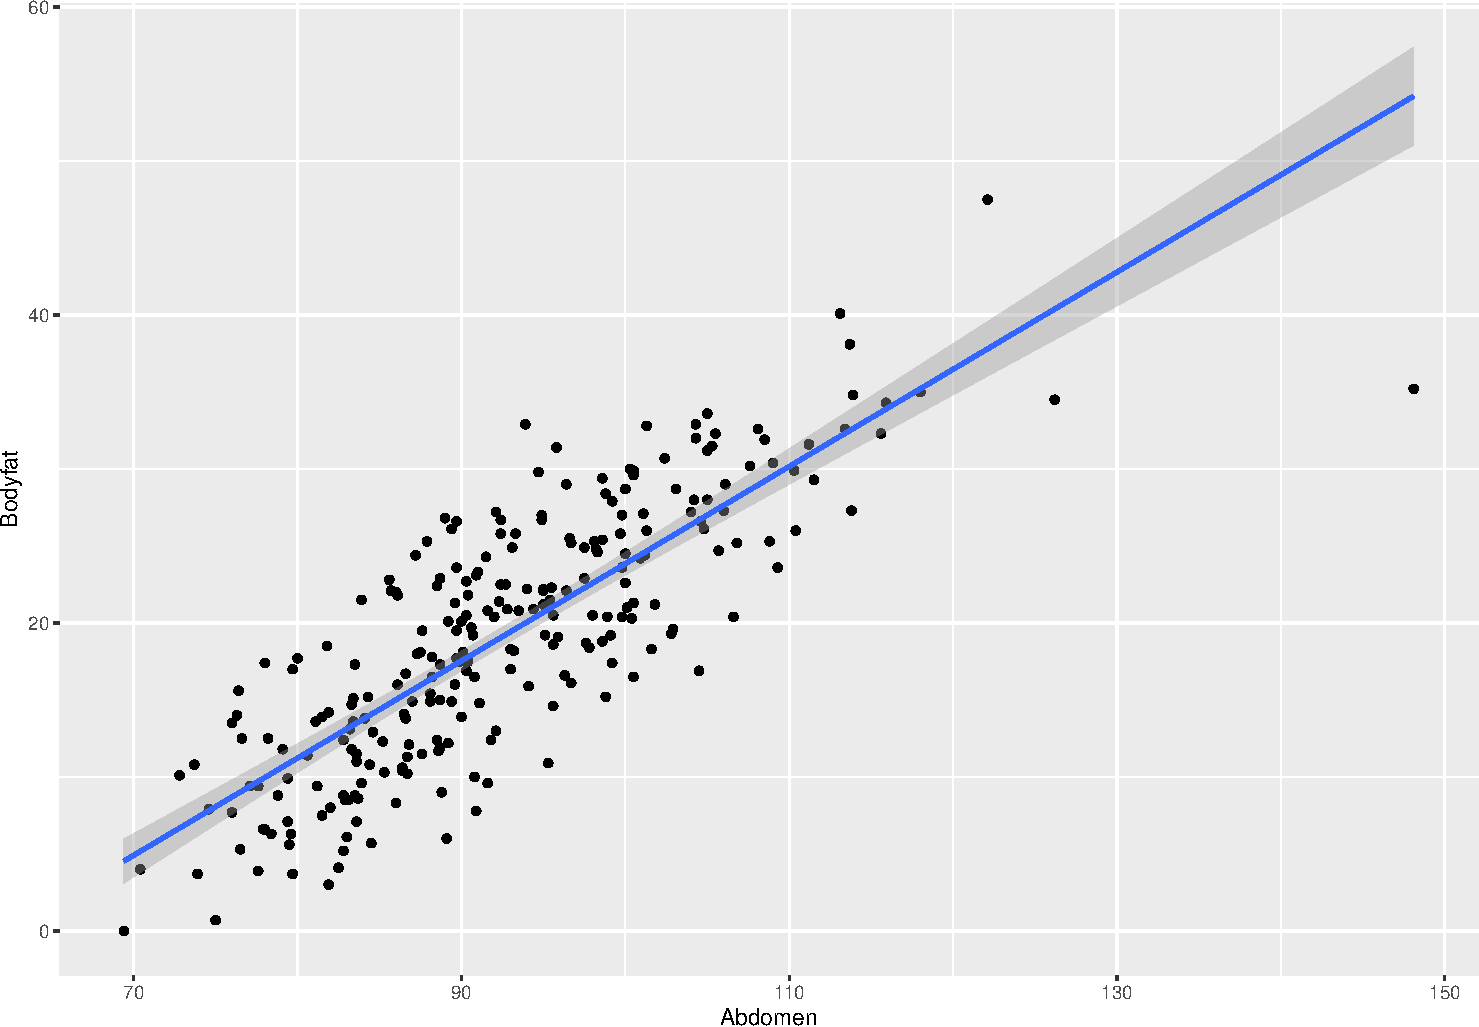
\includegraphics[width=0.6\linewidth]{Part1_intro_files/figure-beamer/unnamed-chunk-4-1} \end{center}
\end{frame}

\begin{frame}{The core}
\protect\hypertarget{the-core-1}{}
\begin{itemize}
\tightlist
\item
  We have observed something.
\item
  We have questions.
\end{itemize}

\begin{center}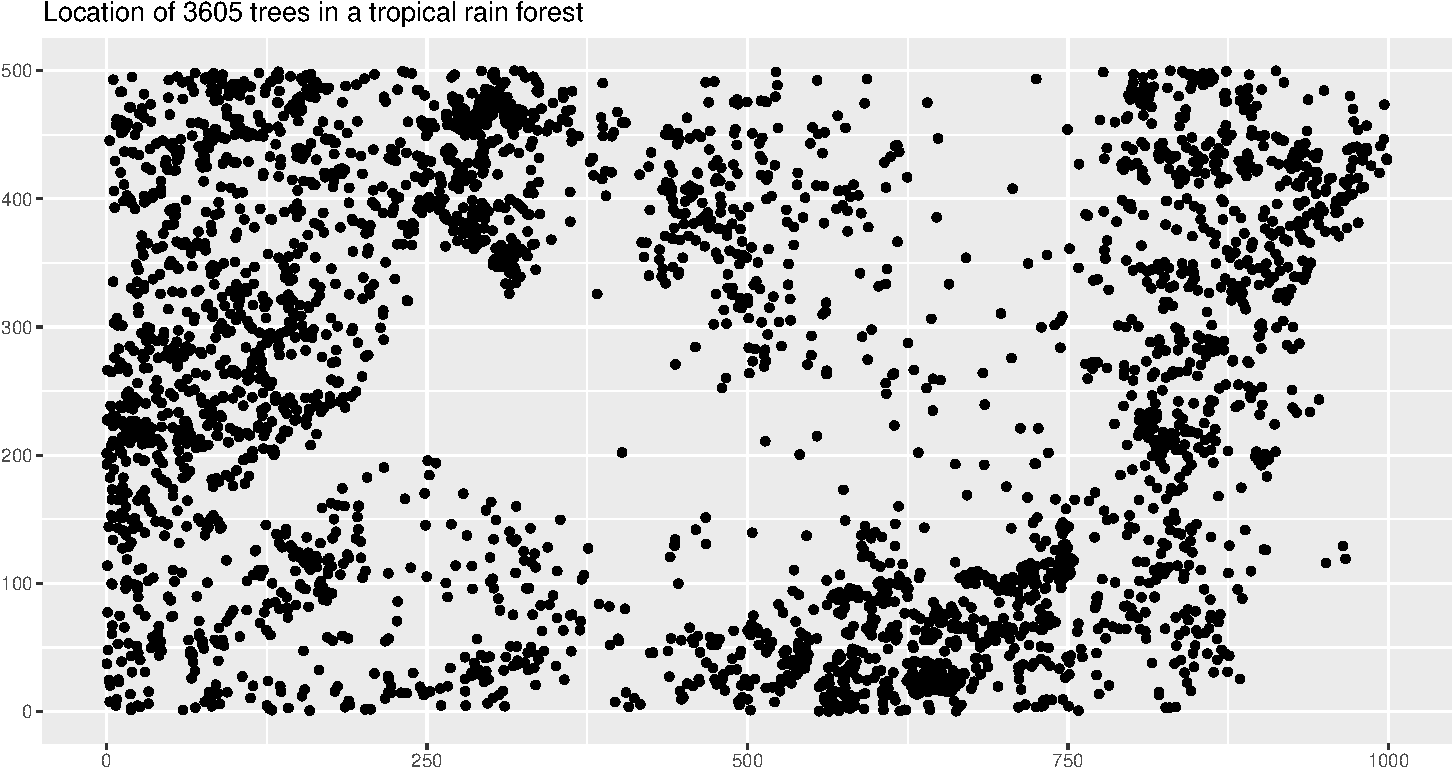
\includegraphics[width=0.6\linewidth]{Part1_intro_files/figure-beamer/unnamed-chunk-5-1} \end{center}
\end{frame}

\begin{frame}{The core}
\protect\hypertarget{the-core-2}{}
\begin{itemize}
\tightlist
\item
  We have observed something.
\item
  We have questions.
\item
  We want answers!
\end{itemize}
\end{frame}

\begin{frame}{How do we find answers?}
\protect\hypertarget{how-do-we-find-answers}{}
We need to make choices:

\begin{itemize}[<+->]
\tightlist
\item
  Bayesian or frequentist?
\item
  How do we model the data?
\item
  \textcolor{red}{How do we compute the answer?}
\end{itemize}

\pause

These questions are \textbf{not} independent.
\end{frame}

\begin{frame}{A simple example}
\protect\hypertarget{a-simple-example}{}
Assume a simple linear regression model with Gaussian observations
\(y = (y_1 , \ldots, y_n)\), where \[
        \text{E}(y_i) = \alpha + \beta x_i,  \text{Var}(y_i) = \tau^{-1}, \quad i=1,\ldots, n
\]

\begin{cols}

\begin{col}{0.55\textwidth}

\begin{center}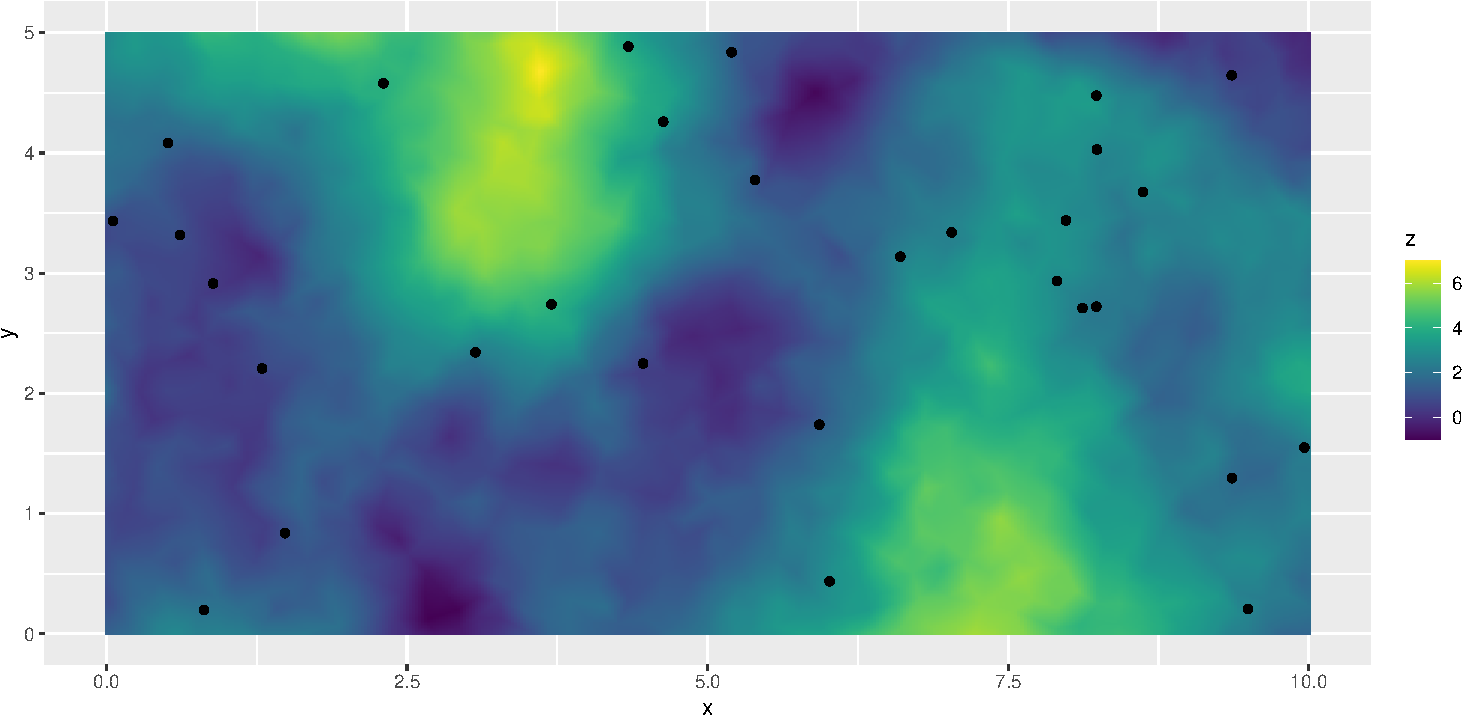
\includegraphics[width=0.9\linewidth]{Part1_intro_files/figure-beamer/unnamed-chunk-6-1} \end{center}

\end{col}

\begin{col}{0.05\textwidth}
~

\end{col}

\begin{col}{0.4\textwidth}

Estimates: \tiny

\begin{longtable}[]{@{}lrl@{}}
\toprule
& Estimate & Std.Error \\
\midrule
\endhead
(Intercept) & -39.280 & 2.66 \\
Abdomen & 0.631 & 0.029 \\
Residual sd & 4.877 & \\
\bottomrule
\end{longtable}

\normalsize

\end{col}

\end{cols}
\end{frame}

\begin{frame}{A Bayesian hyerarchical model}
\protect\hypertarget{a-bayesian-hyerarchical-model}{}
\begin{itemize}
\tightlist
\item
  Observation model
\end{itemize}

\[
y \mid \underbrace{\mu,
            \beta}_{{x}}, \underbrace{\tau}_\theta
\] Encodes information about observed data

\begin{itemize}
\item
  Latent model \(x\): The unobserved process
\item
  Hyperprior for \(\theta\)
\end{itemize}

\pause

From this we can compute the \textcolor{red}{posterior distribution} \[
\pi(x, \theta | y) \propto \pi(y | x,
     \theta) \pi(x) \pi(\theta)
\] and then the corresponding
\textcolor{red}{posterior marginal distributions}.
\end{frame}

\begin{frame}{Results}
\protect\hypertarget{results}{}
\begin{itemize}
\tightlist
\item
  Assign priors to \(\alpha,\beta,\tau\)
\item
  Use Bayes theorem to compute posterior distributions
\end{itemize}

\begin{center}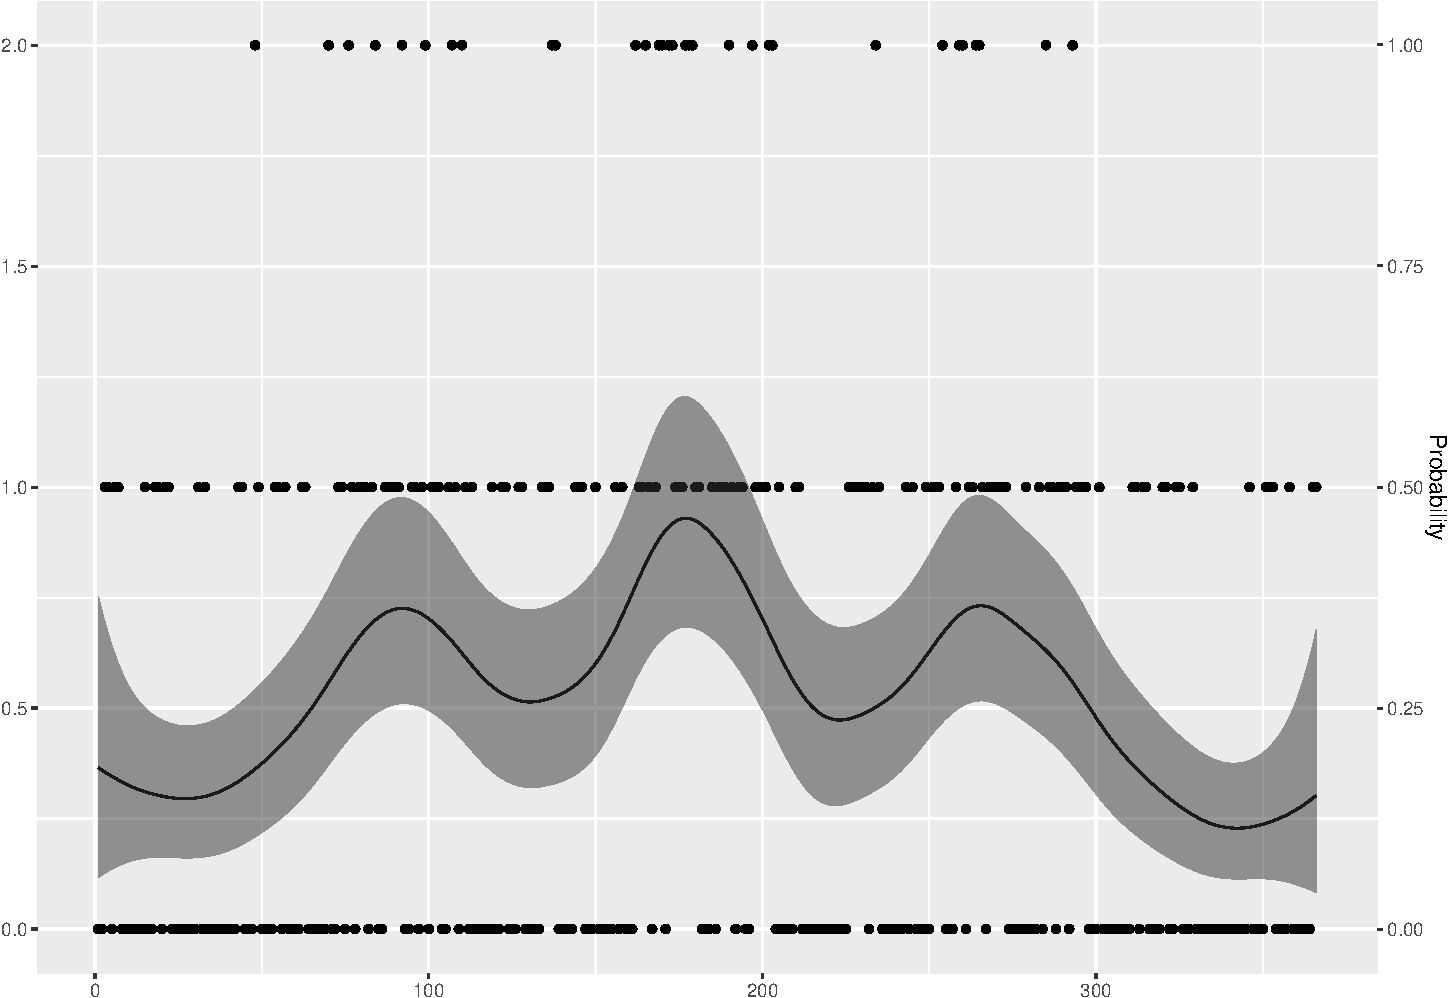
\includegraphics[width=0.6\linewidth]{Part1_intro_files/figure-beamer/unnamed-chunk-9-1} \end{center}
\end{frame}

\hypertarget{bayesian-hierarchical-models}{%
\section{Bayesian hierarchical
models}\label{bayesian-hierarchical-models}}

\begin{frame}{Real-world datasets are usually much more complicated!}
\protect\hypertarget{real-world-datasets-are-usually-much-more-complicated}{}
Using a Bayesian framework:

\begin{itemize}
\tightlist
\item
  Build (hierarchical) models to account for potentially complicated
  dependency structures in the data.
\item
  Attribute uncertainty to model parameters and latent variables using
  priors.
\end{itemize}

\textbf{Two main challenges:}

\begin{enumerate}
\tightlist
\item
  Need computationally efficient methods to calculate posteriors.
\item
  Select priors in a sensible way (see tomorrow)
\end{enumerate}
\end{frame}

\begin{frame}{Bayesian hierarchical models}
\protect\hypertarget{bayesian-hierarchical-models-1}{}
INLA can be used with Bayesian hierarchical models where we model in
different stages or levels:

\begin{itemize}
\tightlist
\item
  \textbf{Stage 1:} What is the distribution of the responses?\\
  \strut \\
\item
  \textbf{Stage 2:} What is the distribution of the underlying
  unobserved (latent) components?\\
  \strut \\
\item
  \textbf{Stage 3:} What are our prior beliefs about the parameters
  controlling the components in the model?
\end{itemize}
\end{frame}

\begin{frame}{Stage 1: The data generating process}
\protect\hypertarget{stage-1-the-data-generating-process}{}
How is our \textcolor{red}{data (\(\boldsymbol{y}\))} generated from the
\textcolor{red}{underlying components  (\(\boldsymbol{x}\))} and
\textcolor{red}{hyperparameters (\(\boldsymbol{\theta}\))} in the model:

\begin{itemize}[<+->]
\tightlist
\item
  Gaussian response? (temperature, rainfall, fish weight \ldots)
\item
  Count data? (people infected with a disease in each area)
\item
  Point pattern? (locations of trees in a forest)
\item
  Binary data? (yes/no response, binary image)
\item
  Survival data? (recovery time, time to death)
\end{itemize}

It is also important how data are collected!\\
\strut \\

This information is placed into our
\textcolor{red}{\textcolor{red}{likelihood}
    \(\pi(\boldsymbol{y} | \boldsymbol{x}, \boldsymbol{\theta})\)}
\end{frame}

\begin{frame}{Stage 1: The data generating process}
\protect\hypertarget{stage-1-the-data-generating-process-1}{}
We assume that \emph{given} the
\textcolor{red}{underlying components    (\(\boldsymbol{x}\))} and
\textcolor{red}{hyperparameters (\(\boldsymbol{\theta}\))} the data are
independent on each other

\[
\pi(y|x,\theta) = \prod_{i\in\cal{I}}\pi(y_i|x_{\cal{I}_i},\theta)
\] \pause

\textcolor{blue}{This implies that all the dependence structure in the data is explained in Stage II !!}
\end{frame}

\begin{frame}{Stage 2: The dependence structure}
\protect\hypertarget{stage-2-the-dependence-structure}{}
The underlying \textcolor{red}{unobserved components \(\boldsymbol{x}\)}
are called \textcolor{red}{\bf{latent} components} and can be:

\begin{itemize}
\tightlist
\item
  Fixed effects for covariates
\item
  Unstructured random effects (individual effects, group effects)
\item
  Structured random effects (AR(1), regional effects, \ldots)
\end{itemize}

These are linked to the responses in the likelihood through linear
predictors.
\end{frame}

\begin{frame}{Stage 3: The hyperparameters}
\protect\hypertarget{stage-3-the-hyperparameters}{}
The likelihood and the latent model typically have hyperparameters that
control their behavior.

The \textcolor{red}{hyperparameters \(\boldsymbol{\theta}\)} can
include:

\pause

\textcolor{red}{Examples likelihood:}

\begin{itemize}
\tightlist
\item
  Variance of observation noise
\item
  Dispersion parameter in the negative binomial model
\item
  Probability of a zero (zero-inflated models)
\end{itemize}

\pause

\textcolor{red}{Examples latent model:}

\begin{itemize}
\tightlist
\item
  Variance of unstructured effects
\item
  Correlation of multivariate effects
\item
  Range and variance of spatial effects
\item
  Autocorrelation parameter
\end{itemize}
\end{frame}

\begin{frame}{Example: Tokyo rainfall data}
\protect\hypertarget{example-tokyo-rainfall-data}{}
Rainfall over 1 mm in the Tokyo area for each calendar day during two
years (1983-84) are registered.

\begin{center}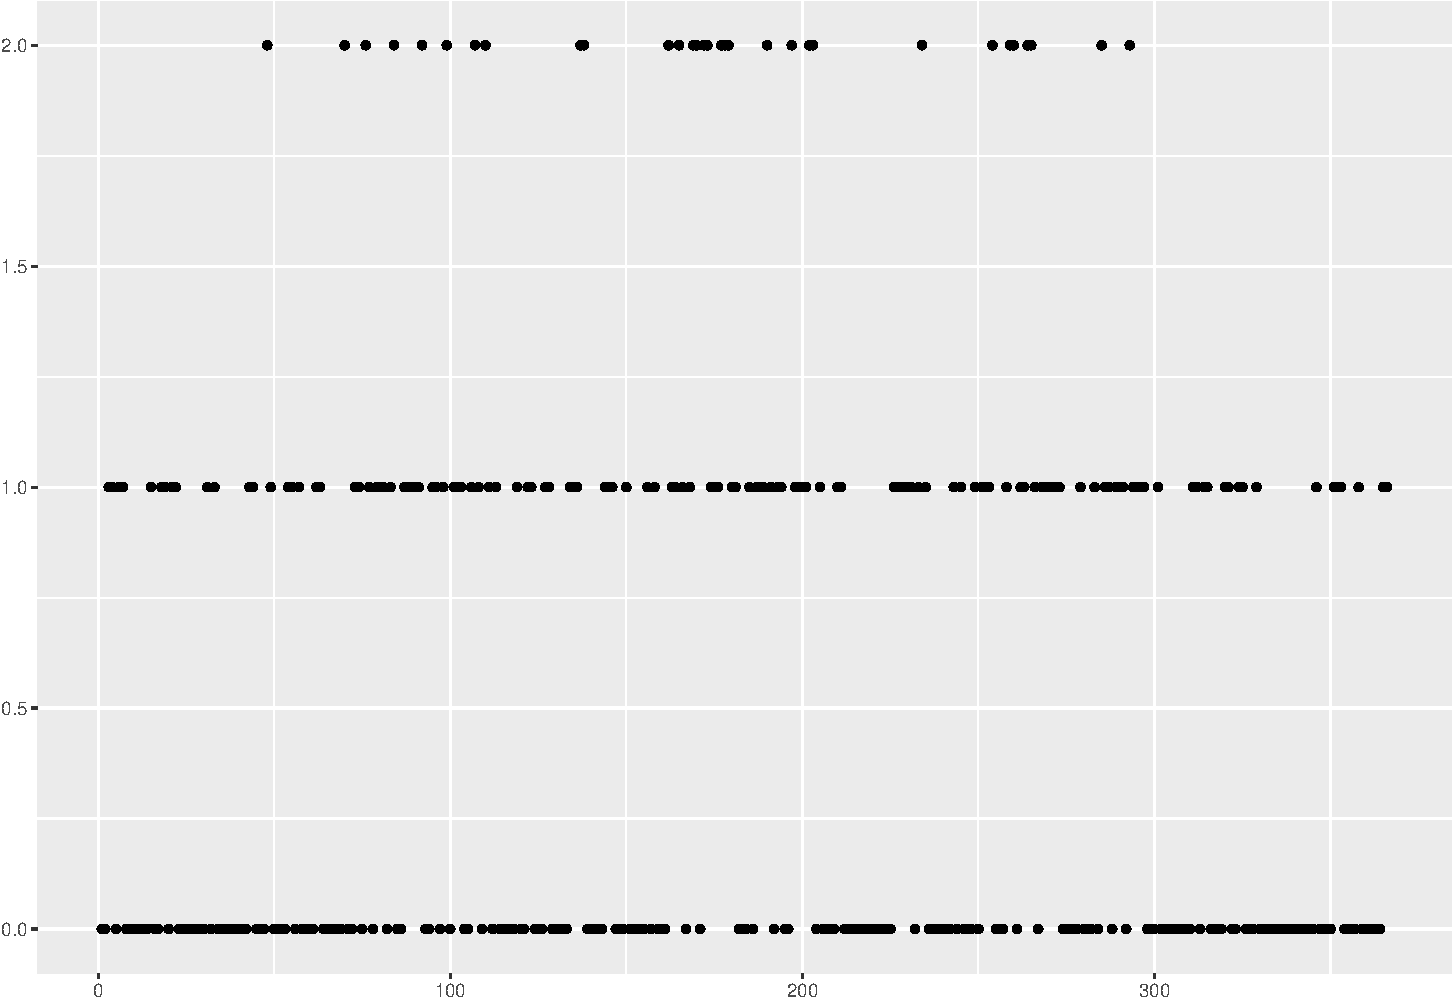
\includegraphics[width=0.6\linewidth]{Part1_intro_files/figure-beamer/unnamed-chunk-10-1} \end{center}
\end{frame}

\begin{frame}{Tokyo rainfall data}
\protect\hypertarget{tokyo-rainfall-data}{}
Rainfall over 1 mm in the Tokyo area for each calendar day during two
years (1983-84) are registered.

\begin{center}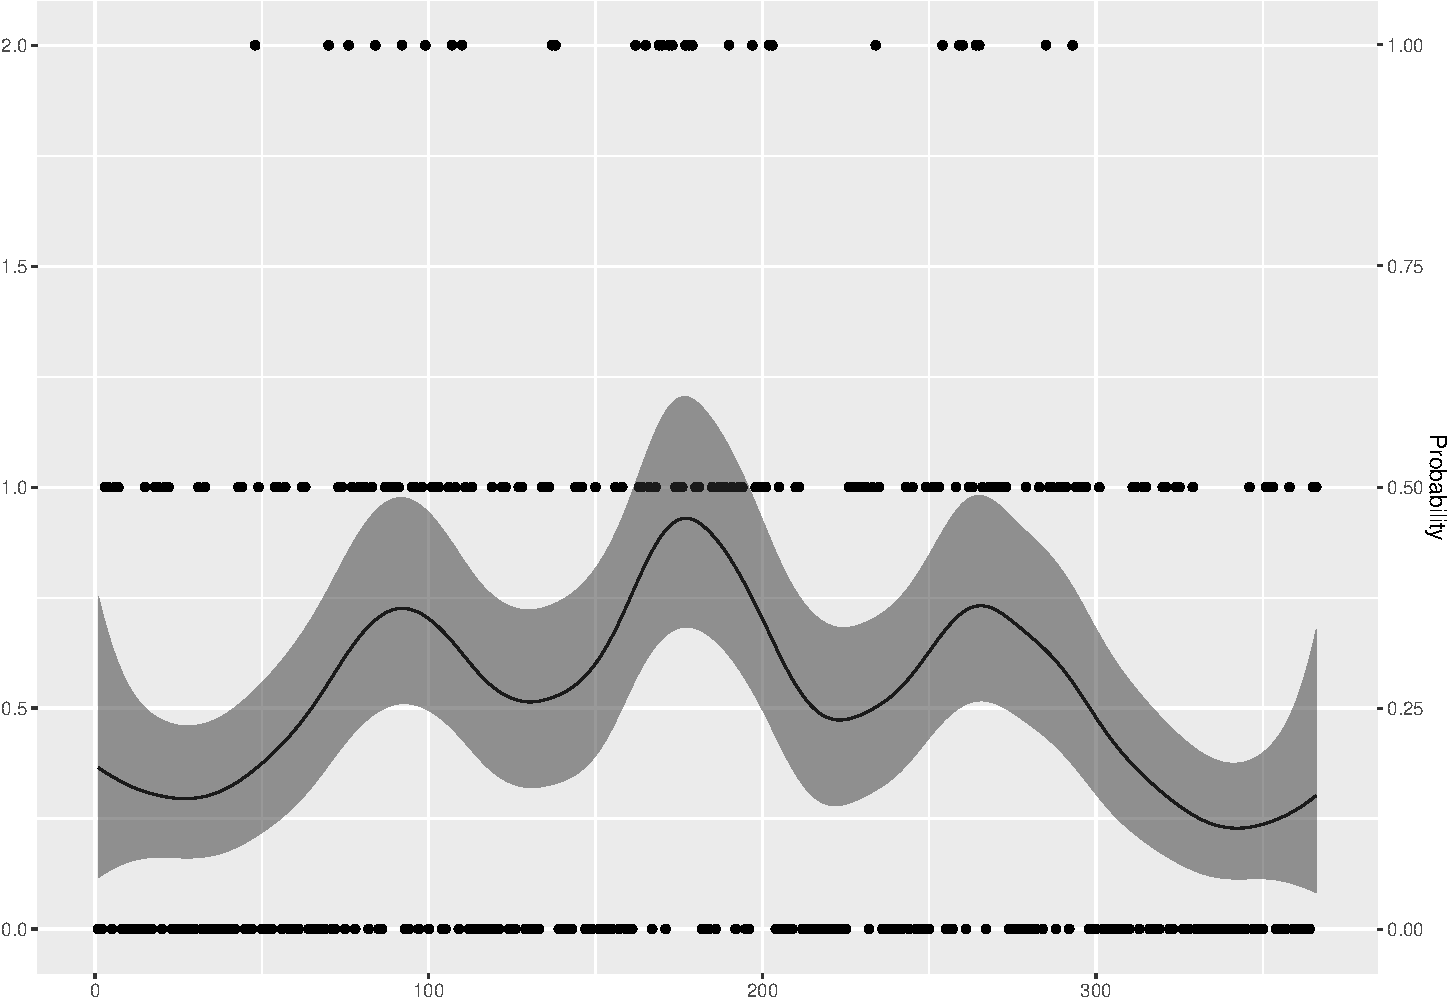
\includegraphics[width=0.6\linewidth]{Part1_intro_files/figure-beamer/unnamed-chunk-11-1} \end{center}
\end{frame}

\begin{frame}{Stage 1: The data}
\protect\hypertarget{stage-1-the-data}{}
\textcolor{red}{
$$
y_i\mid p_i \sim \text{Binomial}(n_i, p_i),
$$} for \(i=1,2,...,366\)

\[
n_{i} = \left\{
 \begin{array}{lr}
1, & \text{for}\; 29\; \text{February}\\
2, & \text{other days}
\end{array}\right.
\] \[
y_{i} =
\begin{cases}
\{0,1\}, & \text{for}\; 29\; \text{February}\\
\{0,1,2\}, & \text{other days}
 \end{cases}       
\]

Linear predictor \[
logit(p_i) = x_i \quad \Leftrightarrow \quad p_i = \frac{1}{1+exp(-x_i)}
\]

\begin{itemize}
\tightlist
\item
  probability of rain on day \(i\) depends on \(x_i\)
\item
  the likelihood has no hyperparameters \(\theta\)
\end{itemize}
\end{frame}

\begin{frame}{Stage 2: The latent model}
\protect\hypertarget{stage-2-the-latent-model}{}
It seems natural borrow strength over time and assume a cyclic smooth
random effect, e.g.~a
\textcolor{red}{cyclic random walk of first or second  order}. A random
walk of first order (CRW1) is defined as:

\[
\begin{aligned}
\pi(x|{\theta})  &\propto 
  \exp\left\{-\frac{\theta}{2}\left[(x_1-x_{366})^2 +
\sum_{i=2}^{366}(x_i-x_{i-1})^2 \right] \right\} \\
 & =  \exp\left\{-\frac{\theta}{2} x^{T}{R}x\right\}
\end{aligned}
\] \pause \scriptsize \[
R = \left[\begin{array}
{rrrrrrrrrr}
2 & -1 & & & &  & & & & -1\\
-1 & 2 & -1 & & & & & & \\
& -1 & 2 & -1 & & & & & \\
& & &  & \ddots & & &  & \\
& & & & & -1 & 2 & -1 &\\
& & & &  & & -1 & 2 & -1 \\
-1 & & & & & & & -1 & 2 \\
\end{array}
\right]
\] \normalsize
\end{frame}

\begin{frame}{Stage 3: Hyperparameters}
\protect\hypertarget{stage-3-hyperparameters}{}
The structured time effect is controlled by one
\textcolor{red}{precision (inverse variance) parameter $\theta$}.

\begin{itemize}
\tightlist
\item
  \textcolor{red}{A larger value of $\theta$ means less variation in $x$},
  i.e.~a smoother effect.
\item
  \(\theta\) is related to the variation in \(p_i\).
\item
  \(\theta > 0\): people commonly assume \[
  \theta \sim \text{Ga}(\text{shape} = a, \text{rate} = b)
  \]
\item
  However, \(\theta\) depends on \({R}\), so it is hard to define values
  for \(a\) and \(b\). You could do this by defining reasonable lower
  and upper quantiles. (We talk about this tomorrow)
\end{itemize}
\end{frame}

\hypertarget{latent-gaussian-models}{%
\section{Latent Gaussian models}\label{latent-gaussian-models}}

\begin{frame}{Latent Gaussian models}
\protect\hypertarget{latent-gaussian-models-1}{}
This was just one example of a very useful class of models called
\textcolor{red}{\bf Latent Gaussian models}.

\begin{itemize}
\tightlist
\item
  The characteristic property is that the \textcolor{red}{latent part}
  of the hierarchical model is
  \textcolor{red}{Gaussian,  \(\boldsymbol{x} | \boldsymbol{\theta} \sim N(0, {Q}^{-1})\)}
\item
  The expected value is \(\boldsymbol{0}\)
\item
  The \emph{precision} matrix (inverse covariance matrix) is \({Q}\)
\end{itemize}
\end{frame}

\begin{frame}{The general set-up}
\protect\hypertarget{the-general-set-up}{}
The set up contains GLMs, GLMMs, GAMs, GAMMs, and more. The mean of the
observation \(i\), \(\mu_i\), is connected to the linear predictor,
\(\eta_i\), through a link function \(g\), \[
\eta_i = g(\mu_i) = \mu + \boldsymbol{z}_i^\top \boldsymbol{\beta}+\sum_{\gamma} w_{\gamma, i} f_\gamma(c_{\gamma,i})+v_i, \quad i = 1,2,\ldots,n
\]

where \[
\begin{aligned}
\mu &: \text{Intercept}\\
        \boldsymbol{\beta} &: \text{Fixed effects of covariates \(\boldsymbol{z}\)}\\
        \{f_\gamma(\cdot)\} &: \text{Non-linear/smooth effects of covariates \(\boldsymbol{c}\)}\\
        \{w_{\gamma,i}\} &: \text{Known weights defined for each observed data point}\\
        \boldsymbol{v} &: \text{Unstructured error terms}
\end{aligned}
\]
\end{frame}

\begin{frame}{Loads of examples}
\protect\hypertarget{loads-of-examples}{}
\begin{itemize}
\tightlist
\item
  Generalized linear and additive (mixed) models
\item
  Disease mapping
\item
  Survival analysis
\item
  Log-Gaussian Cox-processes
\item
  Geostatistics
\item
  Spatio and spatio-temporal models
\item
  Stochastic volatility models
\item
  Measurement error models
\item
  And more!
\end{itemize}
\end{frame}

\begin{frame}{Specification of the latent field}
\protect\hypertarget{specification-of-the-latent-field}{}
\begin{itemize}[<+->]
\tightlist
\item
  Collect all parameters (random variables) in the
  \textcolor{red}{latent field}
  \({x} =\{\mu, {\beta}, \{f_\gamma(\cdot)\}, {\eta}\}\).
\item
  A latent Gaussian model is obtained by assigning Gaussian priors to
  all elements of \({x}\).
\item
  Very flexible due to many different forms of the unknown functions
  \(\{f_\gamma(\cdot)\}\):
\item
  \textcolor{red}{Hyperparameters} account for variability and
  length/strength of dependence
\end{itemize}
\end{frame}

\begin{frame}{Flexibility through \(f\)-functions}
\protect\hypertarget{flexibility-through-f-functions}{}
The functions \(\{f_\gamma\}\) in the linear predictor make it possible
to capture very different types of random effects in the same framework:

\begin{itemize}
\tightlist
\item
  \(f(\texttt{time})\):, For example, an AR(1) process, RW1 or RW2
\item
  \(f(\texttt{spatial location})\):, For example, a Mat'ern field
\item
  \(f(\texttt{covariate})\):, For example, a RW1 or RW2 on the covariate
  values
\item
  \(f(\texttt{time}, \texttt{spatial location})\) can be a
  spatio-temporal effect
\item
  And much more
\end{itemize}
\end{frame}

\begin{frame}{Additivity}
\protect\hypertarget{additivity}{}
\begin{itemize}
\tightlist
\item
  One of the most useful features of the framework is the additivity.
\item
  Effects can easily be removed and added without difficulty.
\item
  Each component might add a new latent part and might add new
  hyperparameters, but the modelling framework and computations stay the
  same.
\end{itemize}

\pause

\textcolor{red}{OBS:} The \emph{linear} predictor needs to stay linear!!
So effects can be added but not multiplied (will say more tomorrow..)
\end{frame}

\begin{frame}{A small point to think about}
\protect\hypertarget{a-small-point-to-think-about}{}
From a Bayesian point of view fixed effects and random effects are all
the same.

\begin{itemize}
\tightlist
\item
  Fixed effects are also random
\item
  They only differ in the prior we put on them
\end{itemize}
\end{frame}

\begin{frame}{Example: disease mapping}
\protect\hypertarget{example-disease-mapping}{}
We observed larynx cancer mortality counts for males in 544 district of
Germany from 1986 to 1990 and want to make a model.

\begin{cols}

\begin{col}{0.55\textwidth}

\begin{itemize}
\tightlist
\item
  \(y_i\): The count at location \(i\).
\item
  \(E_i\): An offset; expected number of cases in district \(i\).
\item
  \(c_i\): A covariate (level of smoking consumption) at \(i\)
\item
  \(\boldsymbol{s}_i\): spatial location \(i\) .
\end{itemize}

\end{col}

\begin{col}{0.05\textwidth}
~

\end{col}

\begin{col}{0.4\textwidth}

\begin{center}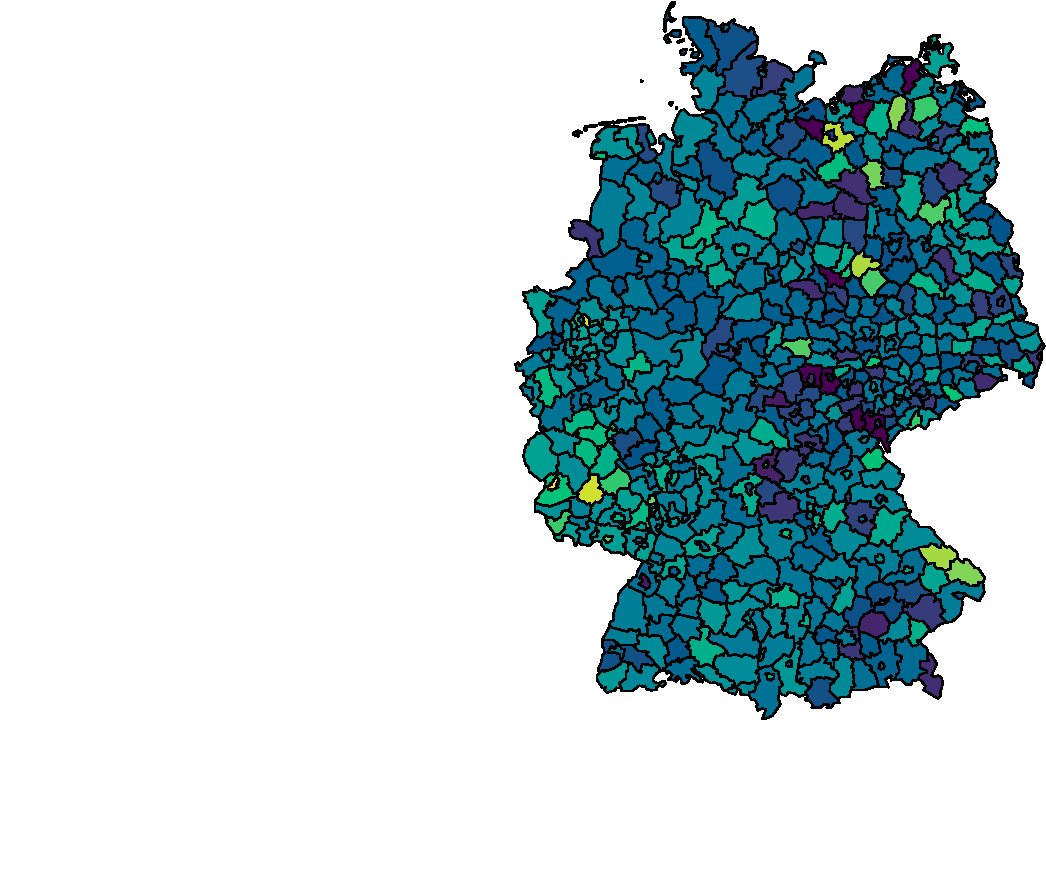
\includegraphics[width=1.1\linewidth]{Part1_intro_files/figure-beamer/unnamed-chunk-12-1} \end{center}

\end{col}

\end{cols}
\end{frame}

\begin{frame}{Bayesian disease mapping}
\protect\hypertarget{bayesian-disease-mapping}{}
\begin{itemize}[<+->]
\tightlist
\item
  \textbf{Stage 1:} We choose a Poisson distribution for the responses,
  so that \[
  y_i \mid \eta_i \sim \text{Poisson}(E_i\exp(\eta_i)))
  \]
\item
  \textbf{Stage 2:} \(\eta_i\) is a linear function of the latent
  components: a covariate \(c_i\), a spatially structured effect
  \(f_u\), an unstructured effect \({v}\) likelihood by \[
  \eta_i = \mu+ \beta c_i + f_u(s_i) + v_i
  \]
\item
  \textbf{Stage 3:}

  \begin{itemize}[<+->]
  \tightlist
  \item
    \(\tau_f\): Precision parameter for the structured effect
  \item
    \(\tau_v\): Precision parameter for the unstructured effect \pause\\
  \end{itemize}
\end{itemize}

The latent field is \textcolor{red}{$\boldsymbol{x} = (\mu, \beta,
        \{f_u(\cdot)\}, v_1, v_2,\ldots, v_n)$}, the hyperparameters are
\textcolor{red}{ $\boldsymbol{\theta} = (\tau_f,\tau_v)$}, and must be
given a prior.
\end{frame}

\begin{frame}{So\ldots which model fit the INLA framework??}
\protect\hypertarget{sowhich-model-fit-the-inla-framework}{}
\begin{enumerate}
\tightlist
\item
  Latent \textbf{Gaussian} model
\item
  The latent field has a sparse precision matrix (Markov properties)
\item
  The data are conditionally independente given the latent field
\item
  The predictor is linear
\end{enumerate}
\end{frame}

\begin{frame}{Quiz!}
\protect\hypertarget{quiz}{}
Assume that, given \(\eta = (\eta_1,\dots,\eta_n)\) the observations
\(y = (y_1,\dots,y_n)\) are independent and Poisson distributed with
parameter \(\lambda_ i = \exp(\eta_i)\) i.e. \[
y_i|\eta_i =\text{Poisson}(\lambda_i); i = 1,\dots,n 
\]\\
\small 1. \(\eta_i=\alpha+\beta x_i+U_i\) where \[
\begin{aligned}
\alpha,\beta & \sim\mathcal{N}(0,1)\\
U_i & \sim \mathcal{N}(0,1) \text{ for } i = 1,\dots,n
\end{aligned}
\] 2. \(\eta_i=\alpha+\beta x_i+V_i\) where \[
\begin{aligned}
\alpha,\beta & \sim\mathcal{N}(0,1)\\
U_i & \sim \text{Bernoulli}(0.4) \text{ for } i = 1,\dots,n
\end{aligned}
\] 3. \(\eta_i=\alpha+\beta x_i\) where \[
\begin{aligned}
\alpha,\beta & \sim\mathcal{N}(0,1)\\
\end{aligned}
\] 4. \(\eta_i=\alpha+\beta x_i + U_iV_i\) where \[
\begin{aligned}
\alpha,\beta & \sim\mathcal{N}(0,1)\\
U_i & \sim \mathcal{N}(0,1) \text{ for } i = 1,\dots,n\\
V_i & \sim \mathcal{N}(0,1) \text{ for } i = 1,\dots,n
\end{aligned}
\] \normalsize
\end{frame}

\hypertarget{deterministic-inference}{%
\section{Deterministic inference}\label{deterministic-inference}}

\begin{frame}{Computations}
\protect\hypertarget{computations}{}
\Large

\hfill\break
\hfill\break
So\ldots{}\\
\strut \\
Now we have a modelling framework\ldots{}\\
\strut \\
But how do we get our answers? \normalsize
\end{frame}

\begin{frame}{What do we care about?}
\protect\hypertarget{what-do-we-care-about}{}
\textcolor{red}{It depends on the problem!}

\begin{itemize}[<+->]
\tightlist
\item
  A single element of the latent field (e.g.the sign or quantiles of a
  fixed effect)
\item
  A linear combination of elements from the latent field (the average
  over an area of a spatial effect, the difference of two effects)
\item
  A single hyperparameter (the correlation)
\item
  A non-linear combination of hyper parameters (animal models)
\item
  Predictions at unobserved locations
\end{itemize}
\end{frame}

\begin{frame}{What do we care about?}
\protect\hypertarget{what-do-we-care-about-1}{}
The most important quantity in Bayesian statistics is
\textcolor{red}{the posterior distribution}: \[
\begin{aligned}
\overbrace{\pi({x}, {\theta}\mid{y})}^{{\text{Posterior}}} &\propto \overbrace{\pi({\theta}) \pi({x}\mid{\theta})}^{{\text{Prior}}} \overbrace{\prod_{i \in \mathcal{I}}\pi(y_i \mid x_i, {\theta})}^{{\text{Likelihood}}}
\end{aligned}
\] from which we can derive the quantities of interest, such as \[
    \begin{aligned}
        {\pi(x_i \mid {y})} &\propto \int \int \pi({x}, {\theta}\mid{y}) d{x}_{-i} d{\theta}\\
        &= {\int \pi(x_i \mid {\theta}, {y}) \pi({\theta} \mid {y}) d{\theta}}
    \end{aligned}
\] or \(\pi(\theta_j\mid {y})\).

These are very high dimensional integrals and are typically not
analytically tractable.
\end{frame}

\begin{frame}{Traditional approach: MCMC}
\protect\hypertarget{traditional-approach-mcmc}{}
MCMC is based on sampling with the goal to
\textcolor{red}{construct a Markov chain with the target posterior as stationary distribution}.

\begin{itemize}
\tightlist
\item
  Extensively used within Bayesian inference since the 1980's.
\item
  Flexible and general, sometimes the only thing we can do!
\item
  A generic tool is available with \texttt{JAGS}/\texttt{OpenBUGS}.
\item
  Tools for specific models are of course available,
  e.g.\textasciitilde{}\texttt{BayesX} and \texttt{stan}.
\item
  Standard MCMC sampler are generally easy-ish to program and are in
  fact implemented in readily available software
\item
  However, depending on the complexity of the problem, their efficiency
  might be limited.
\end{itemize}
\end{frame}

\begin{frame}{Approximate inference}
\protect\hypertarget{approximate-inference}{}
Bayesian inference can (almost) never be done exactly. Some form of
approximation must always be done.

\begin{itemize}
\tightlist
\item
  MCMC ``works'\,' for everything, but it can be incredibly slow
\item
  Is it possible to make a quicker, more specialized inference scheme
  which only needs to work for this limited class of models?
  (specifically LGM)
\end{itemize}
\end{frame}

\begin{frame}{Recall: What is our model framework?}
\protect\hypertarget{recall-what-is-our-model-framework}{}
Latent Gaussian models

\[
\begin{aligned}
y| x, \theta & \sim \prod  \pi(y_i|x_i,\theta) & \\
x|\theta & \sim\mathcal{N}(0,Q(\theta)) & \text{\textcolor{red}{Gaussian!!!}}\\
\theta & \sim\pi(\theta)& \text{Not Gaussian}
\end{aligned}
\]

where the precision matrix \(Q(\theta)\) is sparse. Generally these
``sparse'\,' Gaussian distributions are called
\textcolor{red}{Gaussian Markov random fields} (GMRFs).

The sparseness can be exploited for very quick computations for the
Gaussian part of the model through numerical algorithms for sparse
matrices.
\end{frame}

\begin{frame}{The INLA idea}
\protect\hypertarget{the-inla-idea}{}
Use the properties of the LGM we have defined to approximate the
posterior \textcolor{red}{marginals}

\[
\begin{aligned}
        \pi(x_i \mid \boldsymbol{y})\quad \text{and} \quad \pi(\theta_j \mid \boldsymbol{y})
    \end{aligned}
\]\\
directly.\\
\strut \\
Let us consider a \textcolor{red}{toy example to illustrate the ideas}.
\end{frame}

\begin{frame}{How does INLA work? A toy example}
\protect\hypertarget{how-does-inla-work-a-toy-example}{}
Smoothing noisy observations - Data

We observe some smooth function but our measures are noisy (but we know
the size of such noise!)

\begin{center}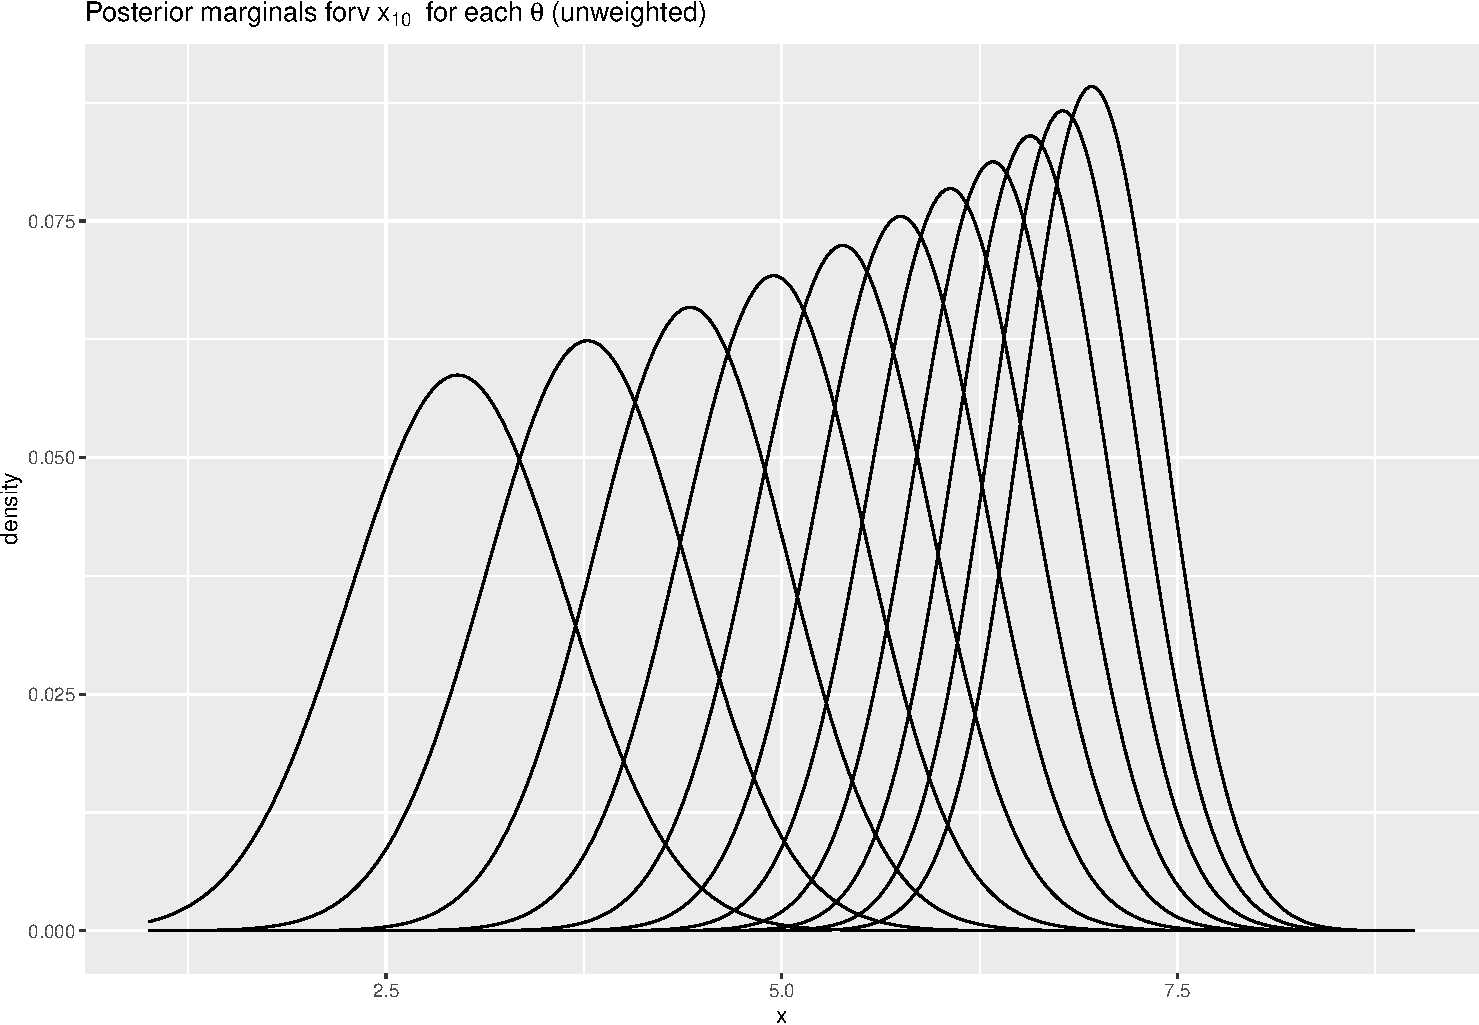
\includegraphics[width=0.6\linewidth]{Part1_intro_files/figure-beamer/unnamed-chunk-13-1} \end{center}

\textbf{Goal:} Recover the smooth function observed with noise!
\end{frame}

\begin{frame}{Smoothing noisy observations - Model}
\protect\hypertarget{smoothing-noisy-observations---model}{}
Assume: \begin{align*}
y_i &= f(i) + \epsilon_i; i = 1,\dots,n \\\nonumber
\epsilon_i&\sim N(0,1) \\\nonumber
f(i) &= x_i\text{ smooth function of } i\nonumber
\end{align*}

\begin{itemize}
\item
  Only one hyperparameter
\item
  Gaussian likelihood
\end{itemize}

\textcolor{red}{Is this a Latent Gaussian model?}
\end{frame}

\begin{frame}{Smoothing noisy observations - LGM}
\protect\hypertarget{smoothing-noisy-observations---lgm}{}
\begin{itemize}
\item
  \textbf{Data} Gaussian Observations with known precision \[
    y_i|x_i\sim\mathcal{N}(x_i,1)
  \]
\item
  \textbf{Latent Model}: A Gaussian model for the smooth function (RW2
  model) \[
    \pi({\bf x}|\theta)\propto \theta^{(n-2)/n}\exp\left\{
    -\frac{\theta}{2}\sum_{i=2}^n(x_i-2x_{i-1}+x_{i-2})^2
    \right\}
  \]
\item
  \textbf{Hyperparameter} The precision of the smooth function
  \(\theta\). We assign a Gamma prior
\end{itemize}

\[
    \pi(\theta)\propto\theta^{a-1}\exp(-b\theta)
\]
\end{frame}

\begin{frame}{Smoothing noisy observations - Goal}
\protect\hypertarget{smoothing-noisy-observations---goal}{}
Find approximations for:

\begin{enumerate}
\tightlist
\item
  The posterior marginal for the hyperparameter \(\pi(\theta|\bf{y})\)
\item
  The posterior marginals for the elements of the latent field
  \(\pi(x_i|\bf{y})\)
\end{enumerate}
\end{frame}

\begin{frame}{Approximating \(\pi(\theta|\bf{y})\)}
\protect\hypertarget{approximating-pithetabfy}{}
We have that \[
    \pi(\bf{x},\theta,\bf{y}) = \pi(\bf{x}|\theta,\bf{y})\pi(\theta|\bf{y})\pi(\bf{y})
\]

so

\[
    \pi(\theta|\bf{y}) = \frac{\pi(\bf{x},\theta,\bf{y})}{\pi(\bf{x}|\theta,\bf{y})\pi(\bf{y})} \propto\frac{
  \pi(\bf{y}, \bf{x}|\theta)\  \pi(\theta)
    }{\pi(\bf{x}|\theta,\bf{y})}
\]

Since the likelihood is Gaussian, then \(\pi(\bf{y}, \bf{x}|\theta)\) is
also Gaussian. We have then:

\[
   \pi(\theta|\bf{y})  \propto \frac{
  \overbrace{\pi(\bf{y}, \bf{x}|\theta)}^{\text{Gaussian}}\  \pi(\theta)}
  {\underbrace{\pi(\bf{x}|\theta,\bf{y})}_{\text{Gaussian}}}
\] This is valid for any \(\bf{x}\)
\end{frame}

\begin{frame}{Posterior marginal for the hyperparameter}
\protect\hypertarget{posterior-marginal-for-the-hyperparameter}{}
Select a grid of points to represent the density \(\pi(\theta|\bf{x})\)

\begin{center}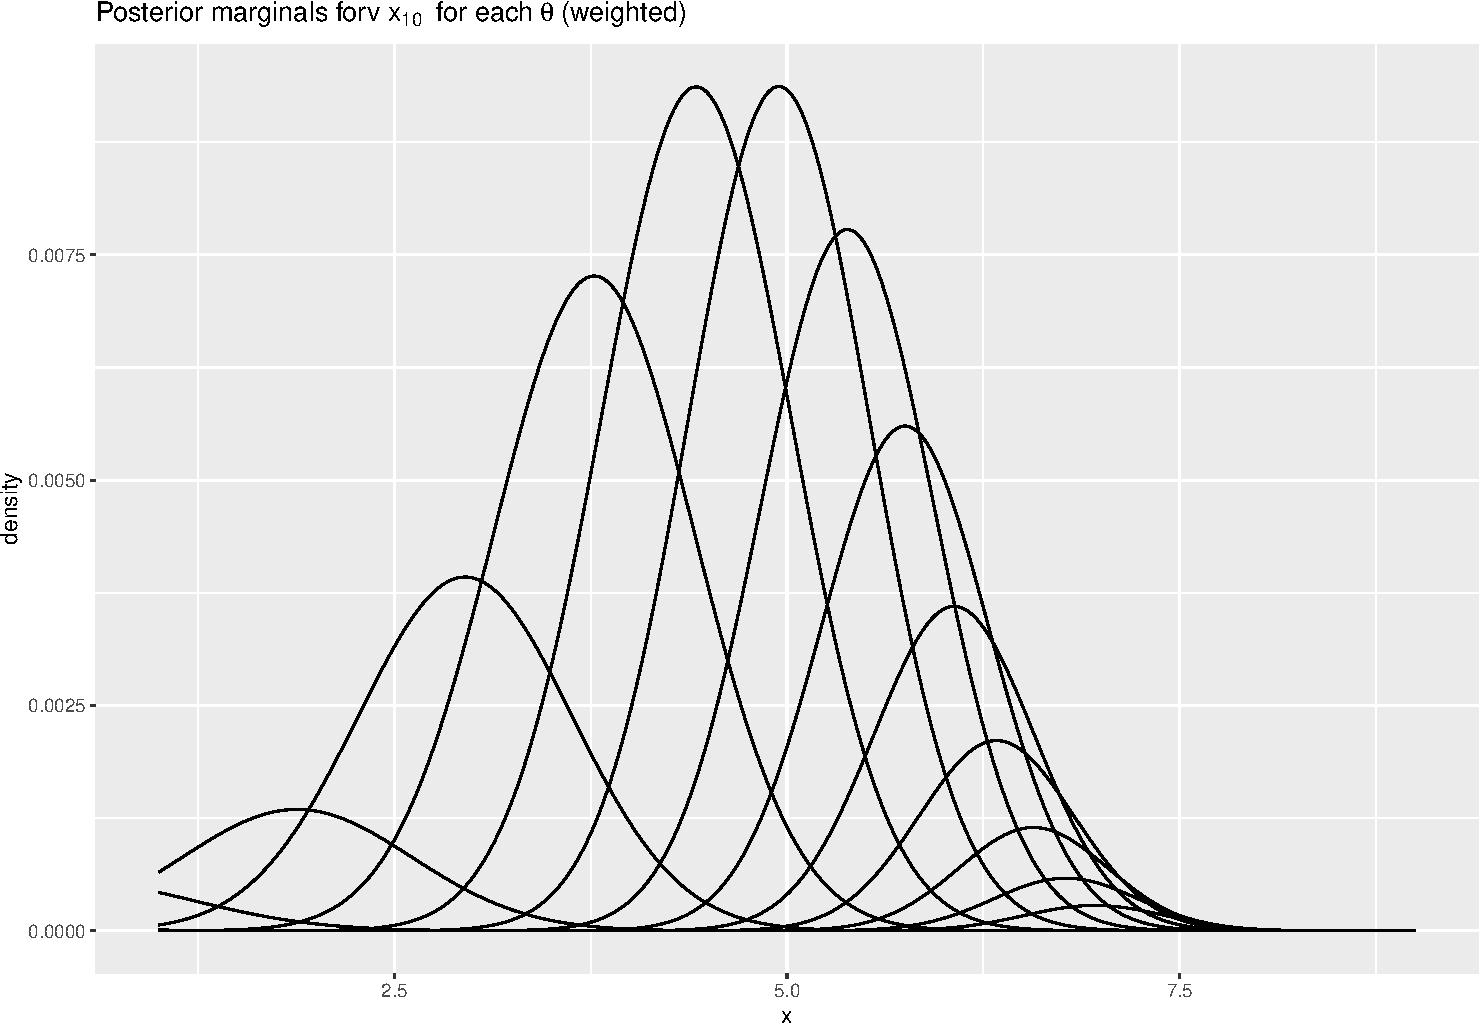
\includegraphics[width=0.6\linewidth]{Part1_intro_files/figure-beamer/unnamed-chunk-14-1} \end{center}
\end{frame}

\begin{frame}{Approximating \(\pi(x_i|y,\theta)\)}
\protect\hypertarget{approximating-pix_iytheta}{}
Again we have that \[
    \bf{x},\bf{y}|\theta\sim\mathbf{N}(\cdot,\cdot)
\] so also \(\pi(x_i|\theta,\bf{y})\) is Gaussian!!\\

We compute \begin{align*}
\pi(x_i|{\bf y}) &= \int \pi(x_i|\theta,{\bf y})\pi(\theta|{\bf y})d\theta\\
      &\approx \sum_k\pi(x_i|\theta_k,{\bf y})\pi(\theta_k|{\bf y}) \Delta_k
\end{align*} where \(\theta_k,k=1,\dots,K\) are the representative
points of \(\pi(\theta|\bf{y})\) and \(\Delta_k\) are the corresponding
weights
\end{frame}

\begin{frame}{Posterior marginals for latent field I}
\protect\hypertarget{posterior-marginals-for-latent-field-i}{}
Compute the conditional posterior marginal for \(x_i\) given each
\(\theta_k\)\\

\begin{center}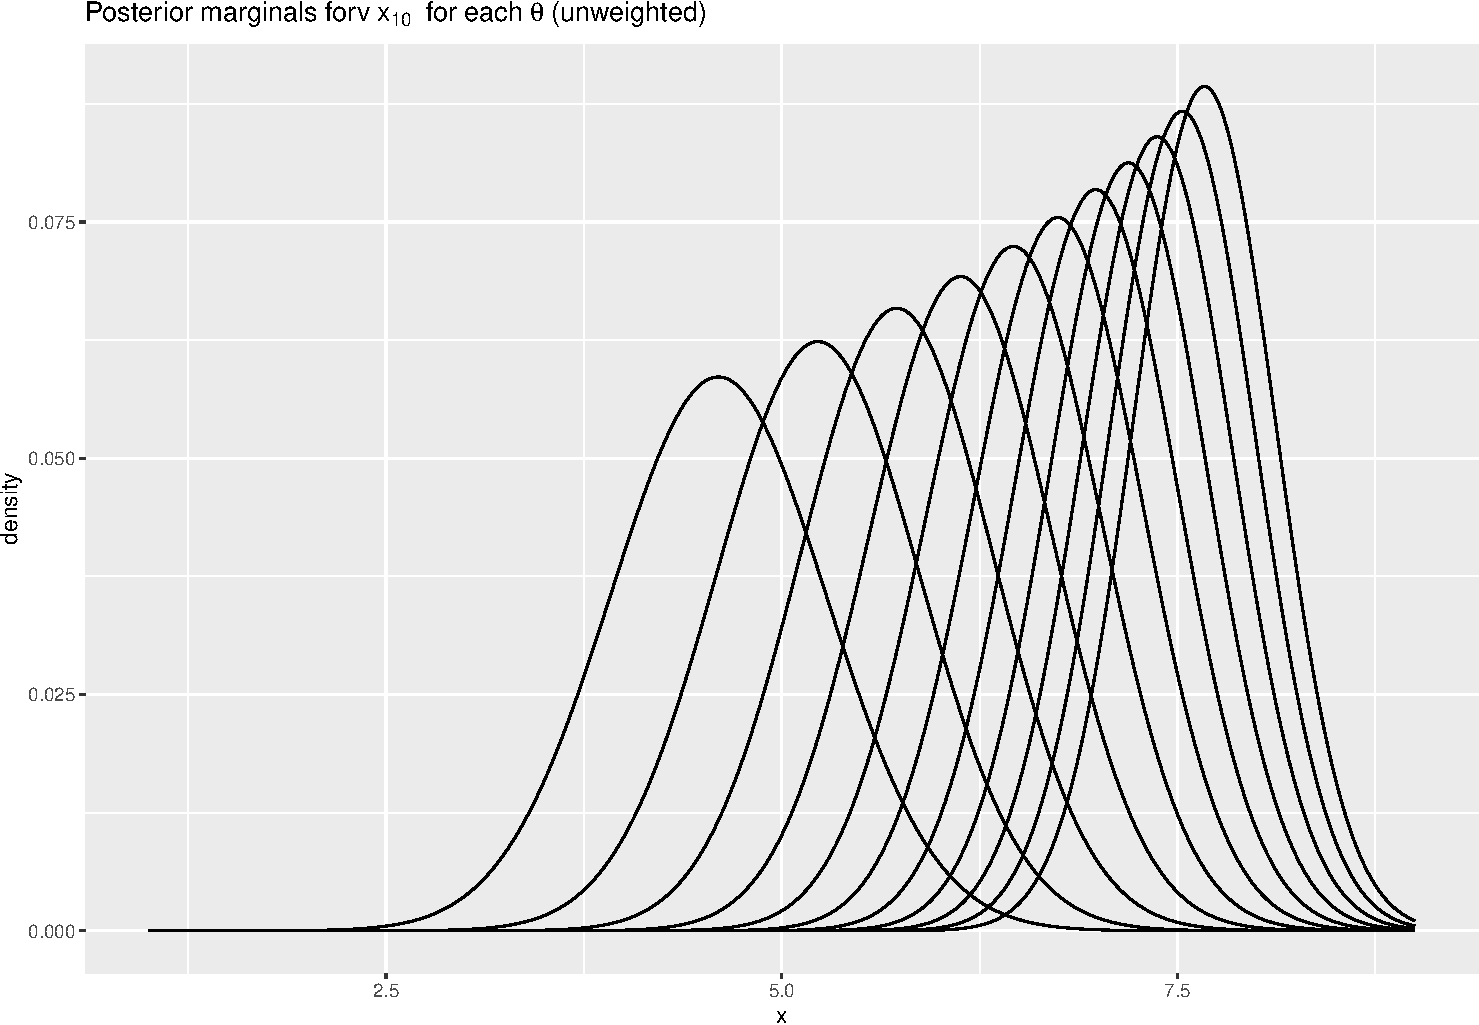
\includegraphics[width=0.6\linewidth]{Part1_intro_files/figure-beamer/unnamed-chunk-15-1} \end{center}
\end{frame}

\begin{frame}{Posterior marginals for latent field II}
\protect\hypertarget{posterior-marginals-for-latent-field-ii}{}
Weight the conditional posterior marginal for
\(\pi(x_i|\theta_k, \bf{y})\) by \(\pi(\theta_k|\bf{y})\Delta_k\)

\begin{center}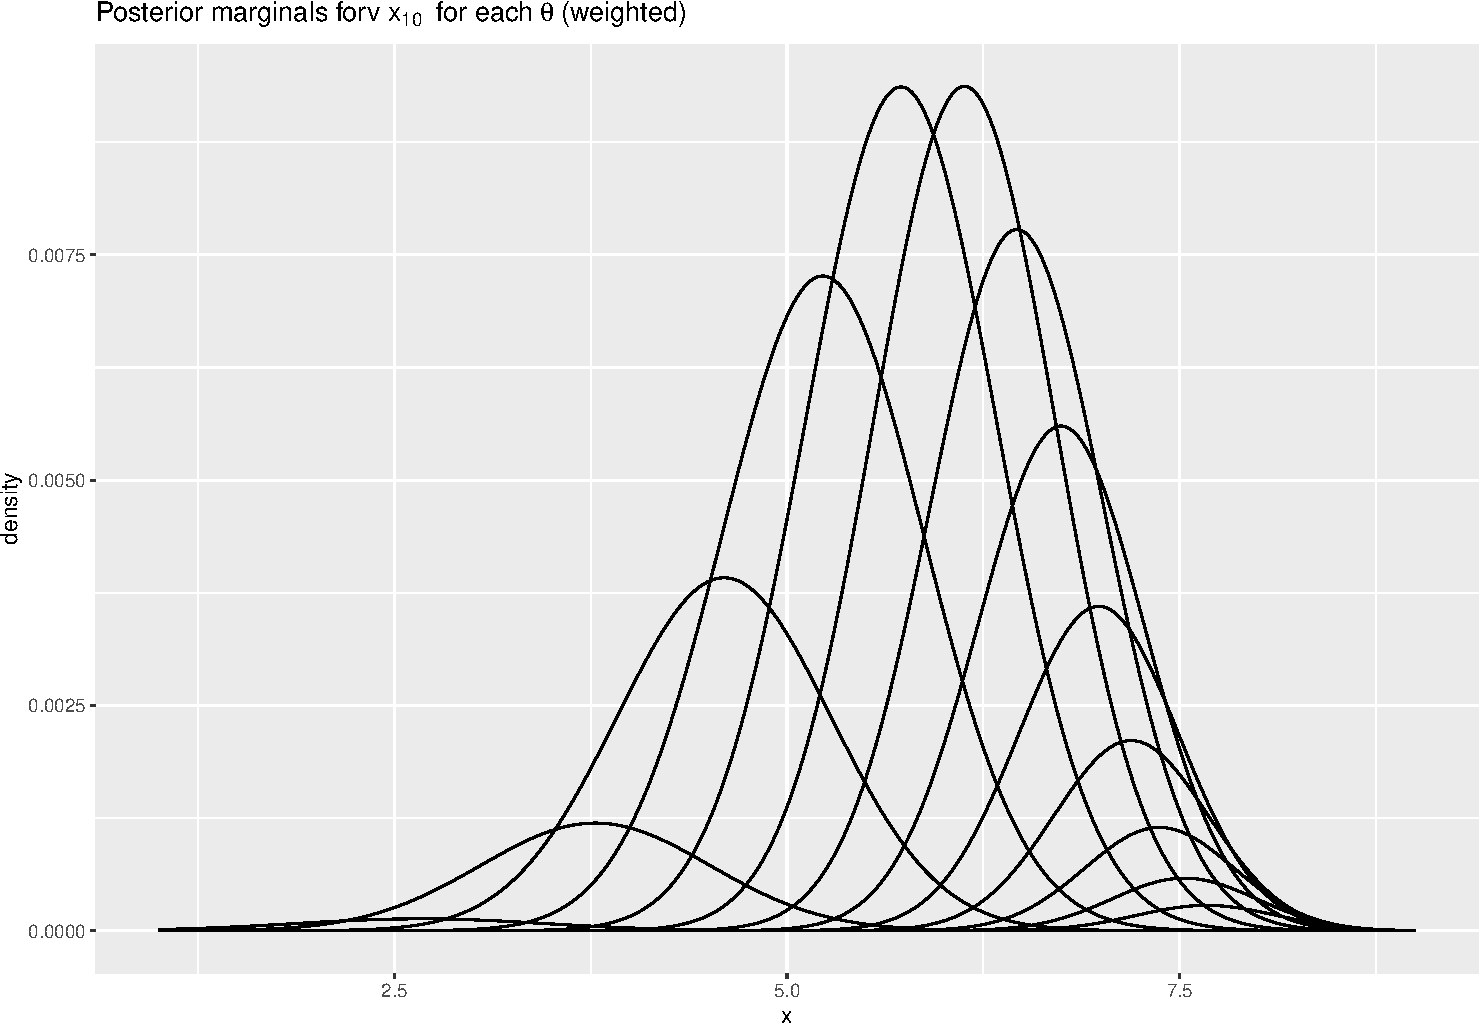
\includegraphics[width=0.6\linewidth]{Part1_intro_files/figure-beamer/unnamed-chunk-16-1} \end{center}
\end{frame}

\begin{frame}{Posterior marginals for latent field III}
\protect\hypertarget{posterior-marginals-for-latent-field-iii}{}
Sum to get the posterior marginal for \(x_i|\bf{y}\)

\begin{center}\includegraphics[width=0.6\linewidth]{Part1_intro_files/figure-beamer/unnamed-chunk-17-1} \end{center}
\end{frame}

\begin{frame}{Fitted Spline}
\protect\hypertarget{fitted-spline}{}
The posterior marginals are used to calculate summary statistics, like
means, variances and credible intervals:

\begin{center}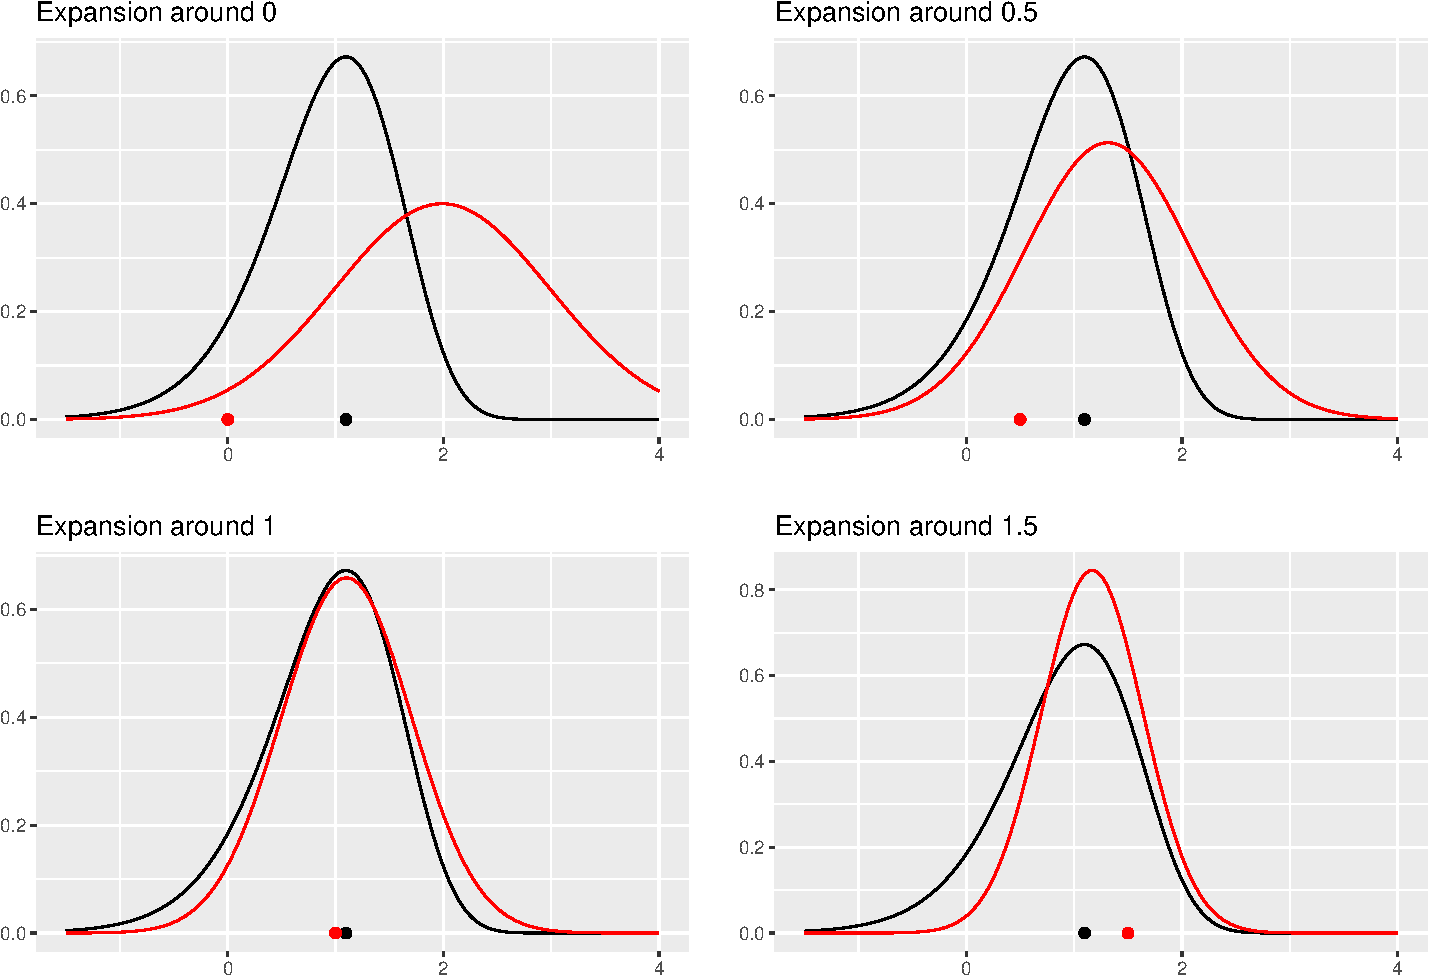
\includegraphics[width=0.6\linewidth]{Part1_intro_files/figure-beamer/unnamed-chunk-18-1} \end{center}
\end{frame}

\begin{frame}[fragile]{\texttt{R-INLA} code}
\protect\hypertarget{r-inla-code}{}
\small

\begin{Shaded}
\begin{Highlighting}[]
\NormalTok{formula }\OtherTok{=}\NormalTok{ y }\SpecialCharTok{\textasciitilde{}} \SpecialCharTok{{-}}\DecValTok{1} \SpecialCharTok{+} \FunctionTok{f}\NormalTok{(idx, }\AttributeTok{model=}\StringTok{"rw2"}\NormalTok{, }\AttributeTok{constr=}\ConstantTok{FALSE}\NormalTok{,}
   \AttributeTok{hyper=}\FunctionTok{list}\NormalTok{(}\AttributeTok{prec=}\FunctionTok{list}\NormalTok{(}\AttributeTok{prior=}\StringTok{"loggamma"}\NormalTok{, }\AttributeTok{param=}\FunctionTok{c}\NormalTok{(a,b))))}

\NormalTok{result }\OtherTok{=} \FunctionTok{inla}\NormalTok{(formula,}
      \AttributeTok{data =} \FunctionTok{data.frame}\NormalTok{(}\AttributeTok{y=}\NormalTok{y, }\AttributeTok{idx=}\NormalTok{idx),}
      \AttributeTok{control.family =} \FunctionTok{list}\NormalTok{(}\AttributeTok{initial =} \FunctionTok{log}\NormalTok{(tau\_0), }\AttributeTok{fixed=}\ConstantTok{TRUE}\NormalTok{))}
\end{Highlighting}
\end{Shaded}

\normalsize
\end{frame}

\begin{frame}{Extending the method}
\protect\hypertarget{extending-the-method}{}
This is the basic idea behind INLA. It is quite simple.

However, we need to extend this basic idea so we can deal with

\begin{enumerate}
\item
  Non-Gaussian observations
\item
  More than one hyperparameter
\end{enumerate}
\end{frame}

\begin{frame}{1. More than one hyperparameter}
\protect\hypertarget{more-than-one-hyperparameter}{}
\textcolor{red}{Main use:} Select good evaluation points \({\theta}_k\)
for the numerical integration when approximating
\(\widetilde{\pi}(x_i|{y})\)

\begin{itemize}
\tightlist
\item
  Locate the mode 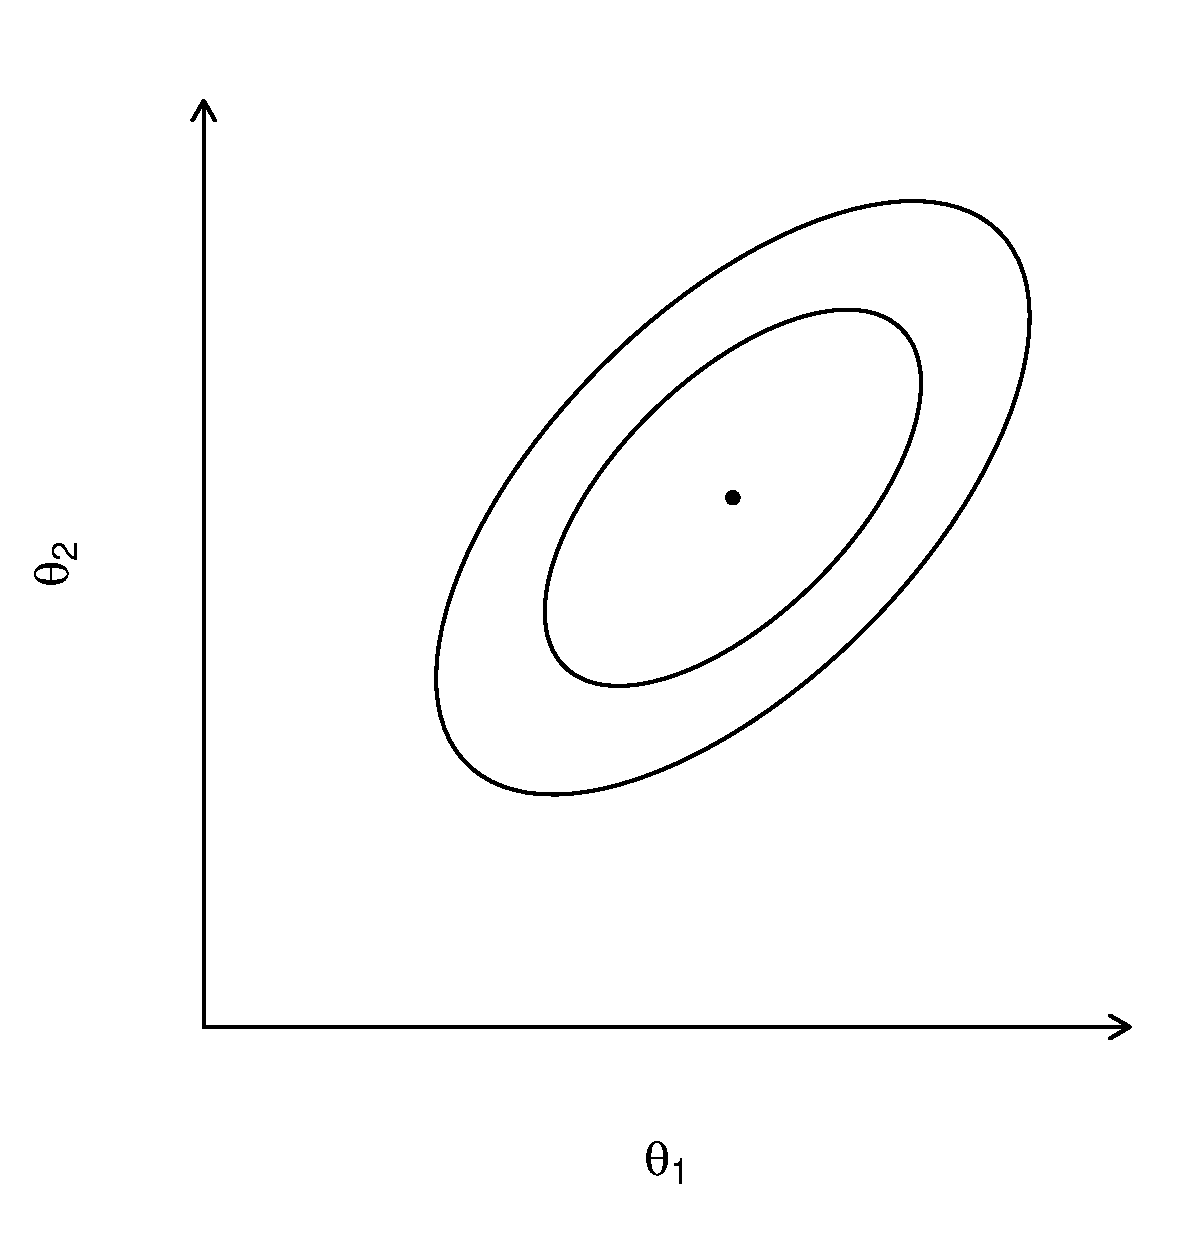
\includegraphics[width=5cm]{./graphics/ellipse1}
\end{itemize}
\end{frame}

\begin{frame}{1. More than one hyperparameter}
\protect\hypertarget{more-than-one-hyperparameter-1}{}
\textcolor{red}{Main use:} Select good evaluation points \({\theta}_k\)
for the numerical integration when approximating
\(\widetilde{\pi}(x_i|{y})\)

\begin{itemize}
\tightlist
\item
  Locate the mode
\item
  Compute the Hessian to construct principal components
  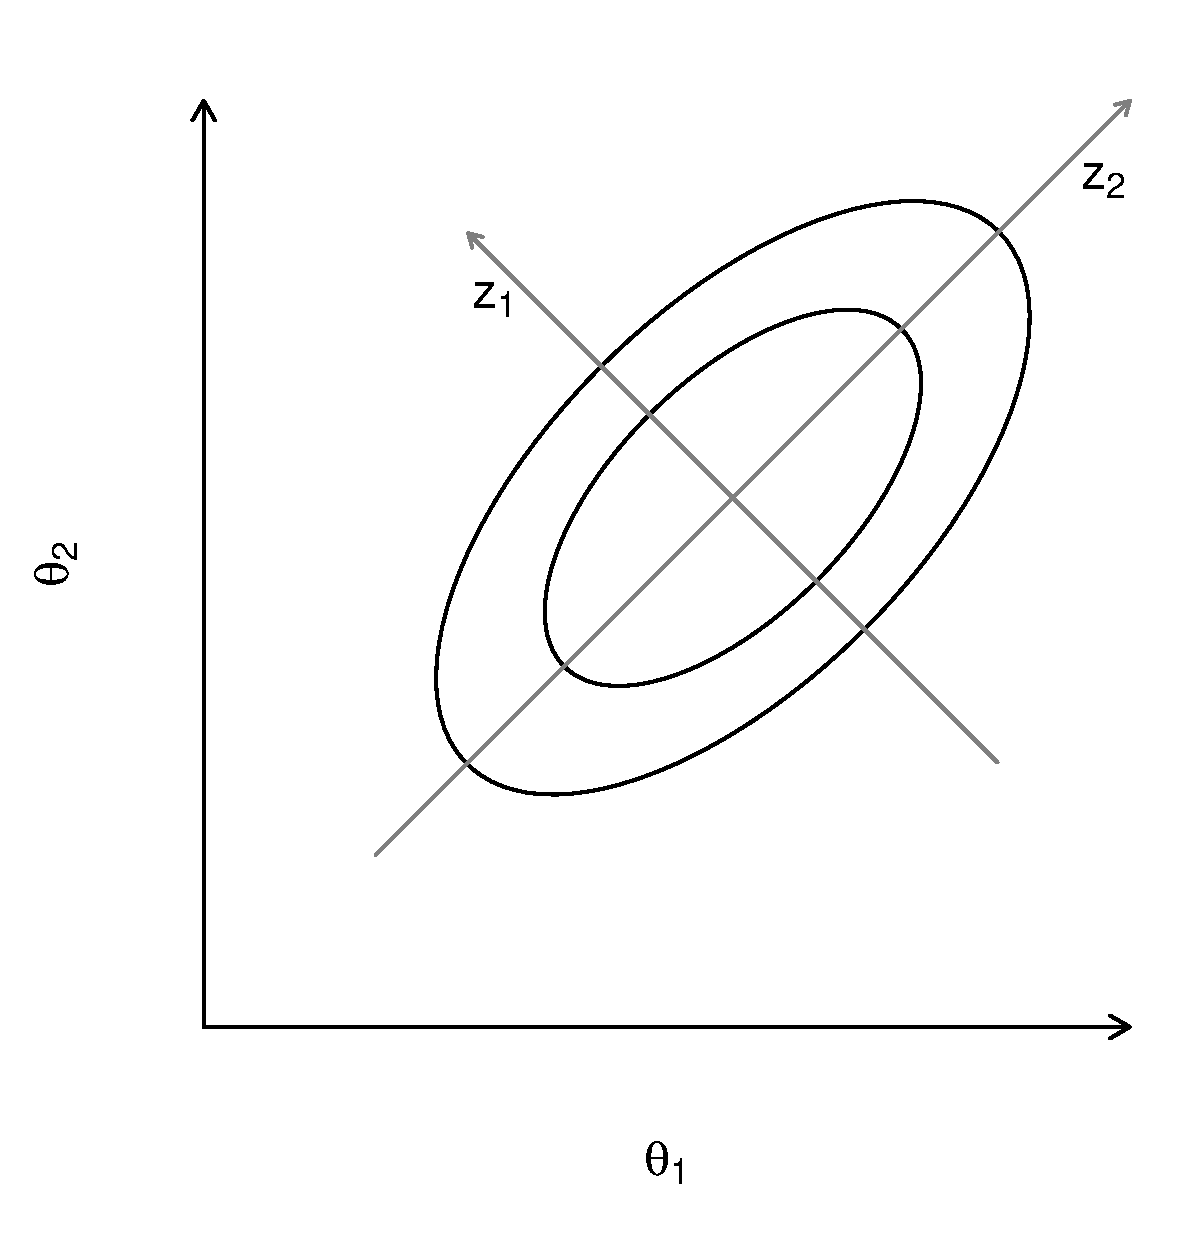
\includegraphics[width=5cm]{./graphics/ellipse2}
\end{itemize}
\end{frame}

\begin{frame}{1. More than one hyperparameter}
\protect\hypertarget{more-than-one-hyperparameter-2}{}
\textcolor{red}{Main use:} Select good evaluation points \({\theta}_k\)
for the numerical integration when approximating
\(\widetilde{\pi}(x_i|{y})\)

\begin{itemize}
\item
  Locate the mode
\item
  Compute the Hessian to construct principal components
\item
  Grid-search to locate bulk of the probability mass
  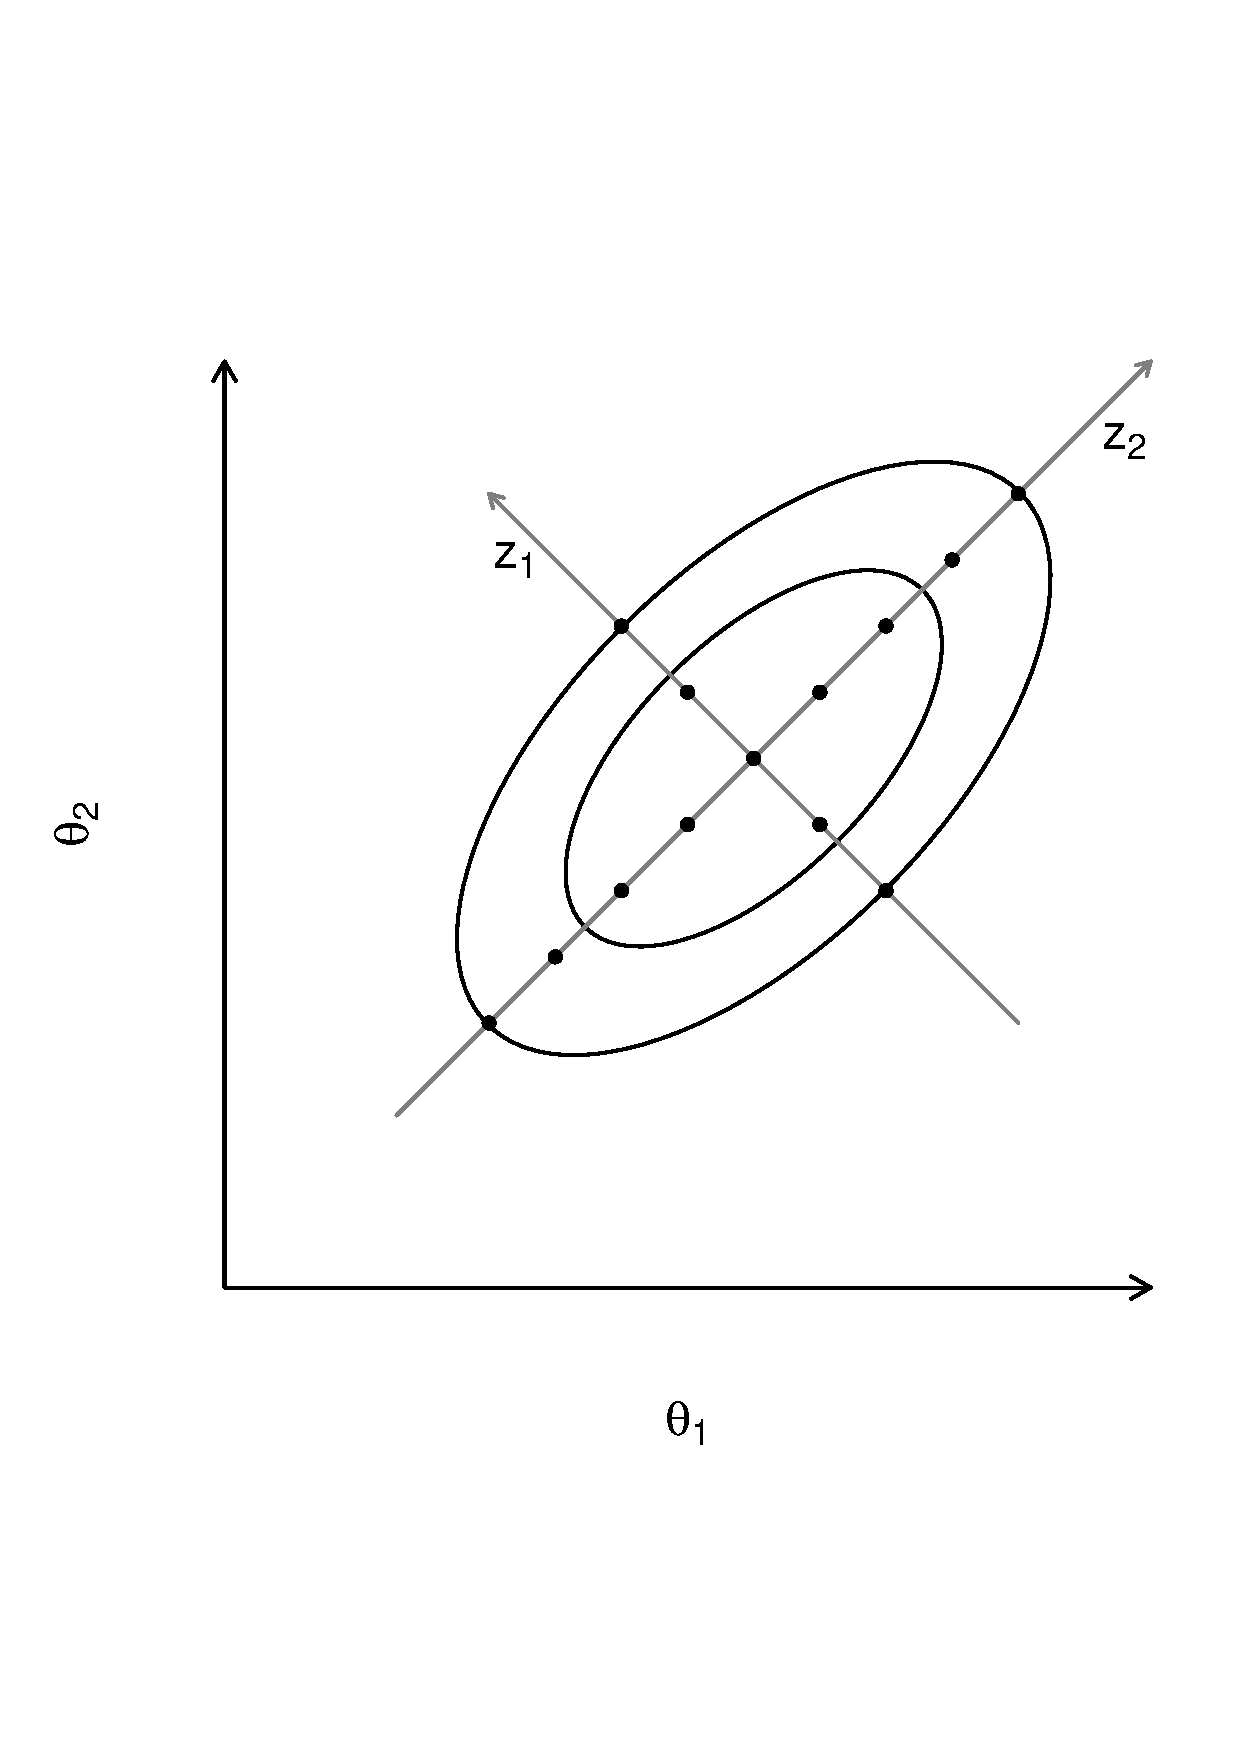
\includegraphics[width=5cm]{./graphics/ellipse3}
\end{itemize}
\end{frame}

\begin{frame}{1. More than one hyperparameter}
\protect\hypertarget{more-than-one-hyperparameter-3}{}
\begin{itemize}
\item
  Locate the mode
\item
  Compute the Hessian to construct principal components
\item
  Grid-search to locate bulk of the probability mass
\item
  For each point \(k\) in the grid compute:

  \begin{itemize}
  \tightlist
  \item
    \(\widetilde{\pi}(\theta^k|y)\)
  \item
    \(\widetilde{\pi}(x_i|\theta^k,y)\)
  \item
    \(\Delta_k\)
  \end{itemize}
\end{itemize}
\end{frame}

\begin{frame}{2. Non-Gaussian observations}
\protect\hypertarget{non-gaussian-observations}{}
In application we may choose likelihoods other than a Gaussian. How does
this change things?

\[
\pi(\bf{\theta} \mid \bf{y}) \propto \frac{
            \overbrace{\pi(\bf{x}, \bf{y}\mid \bf{\theta})}^{\text{Non-Gaussian, BUT KNOWN}}
        \; \pi(\bf{\theta})}{\underbrace{\pi(\bf{x} \mid \bf{y},
            \bf{\theta})}_{\text{Non-Gaussian and UNKNOWN}}}
\]

\begin{itemize}
\tightlist
\item
  In many cases
  \(\pi(\boldsymbol{x} \mid \boldsymbol{y}, \boldsymbol{\theta})\)is
  very close to a Gaussian distribution, and can be replaced with a
  \textcolor{red}{Laplace approximation}.
\end{itemize}
\end{frame}

\begin{frame}{The GMRF (Laplace) approximation}
\protect\hypertarget{the-gmrf-laplace-approximation}{}
Let \(\bf{x}\) denote a GMRF with precision matrix \(\bf{Q}\) and mean
\(\bf{\mu}\).

Approximate \[
\begin{aligned}
\pi(\bf{x}|\theta,\bf{y}) &\propto
            \exp\left(-\frac{1}{2}\bf{x}^\top \bf{Q}\bf{x} + \sum_{i=1}^n \log \pi (y_i|x_i)\right)
\end{aligned}
\] by using a second-order Taylor expansion of \(\log \pi (y_i|x_i)\)
around \(\bf{\mu}_0\), say.

\begin{itemize}
\tightlist
\item
  Recall
\end{itemize}

\[
\begin{aligned}
        f(x) \approx f(x_0) + f'(x_0)(x-x_0)+ \frac{1}{2} f''(x_0)(x-x_0)^2
        = a+ bx - \frac{1}{2}cx^2
\end{aligned}
\] with \(b=f'(x_0) - f''(x_0)x_0\) and \(c = -f''(x_0)\). (Note: \(a\)
is not relevant).
\end{frame}

\begin{frame}{The GMRF approximation (II)}
\protect\hypertarget{the-gmrf-approximation-ii}{}
Thus, \[
\begin{aligned}
        \widetilde{\pi}(\bf{x}|\bf{\theta}, \bf{y}) &\propto
            \exp\left(-\frac{1}{2}\bf{x}^\top \bf{Q}\bf{x}  +
            \sum_{i=1}^n (a_i + b_i x_i - 0.5 c_i x_i^2)\right)\\
        &{\propto \exp\left(-\frac{1}{2}\bf{x}^T(\bf{Q} + \text{diag}(\bf{c})) \bf{x} + \bf{b}^T\bf{x}\right)}
\end{aligned}
\]

which is Gaussian with precision matrix \(\bf{Q} + \text{diag}(\bf{c})\)
and mean given by the solution of
\((\bf{Q} + \text{diag}(\bf{c}))\bf{\mu} = \bf{b}\)

\textcolor{red}{The canonical parameterisation} is \[
\textcolor{red}{\mathcal{N}_C(\mathbf{b}, \bf{Q} + \text{diag}(\bf{c}))}
\] which corresponds to \[
\mathcal{N}((\bf{Q} + \text{diag}(\bf{c}))^{-1}\mathbf{b}, (\bf{Q} + \text{diag}(\bf{c}))^{-1}).
\]
\end{frame}

\begin{frame}{The GMFR approximation - One dimensional example}
\protect\hypertarget{the-gmfr-approximation---one-dimensional-example}{}
Assume \[
\begin{aligned}
  y|\lambda \sim\text{Poisson}(\lambda)  & \text{ Likelihood}\\
  \lambda = \exp(x)  & \text{ Likelihood}\\
  x\sim\mathcal{N}(0,1) & \text{ Latent Model}
\end{aligned}
\] we have that \[
  \pi(x|y)\propto\pi(y|x)\pi(x)\propto\exp\{ -\frac{1}{2}x^2+
  \underbrace{xy-\exp(x)}_{\text{non-gaussian part}}
  \}
\]
\end{frame}

\begin{frame}{The GMRF approximation}
\protect\hypertarget{the-gmrf-approximation}{}
\begin{center}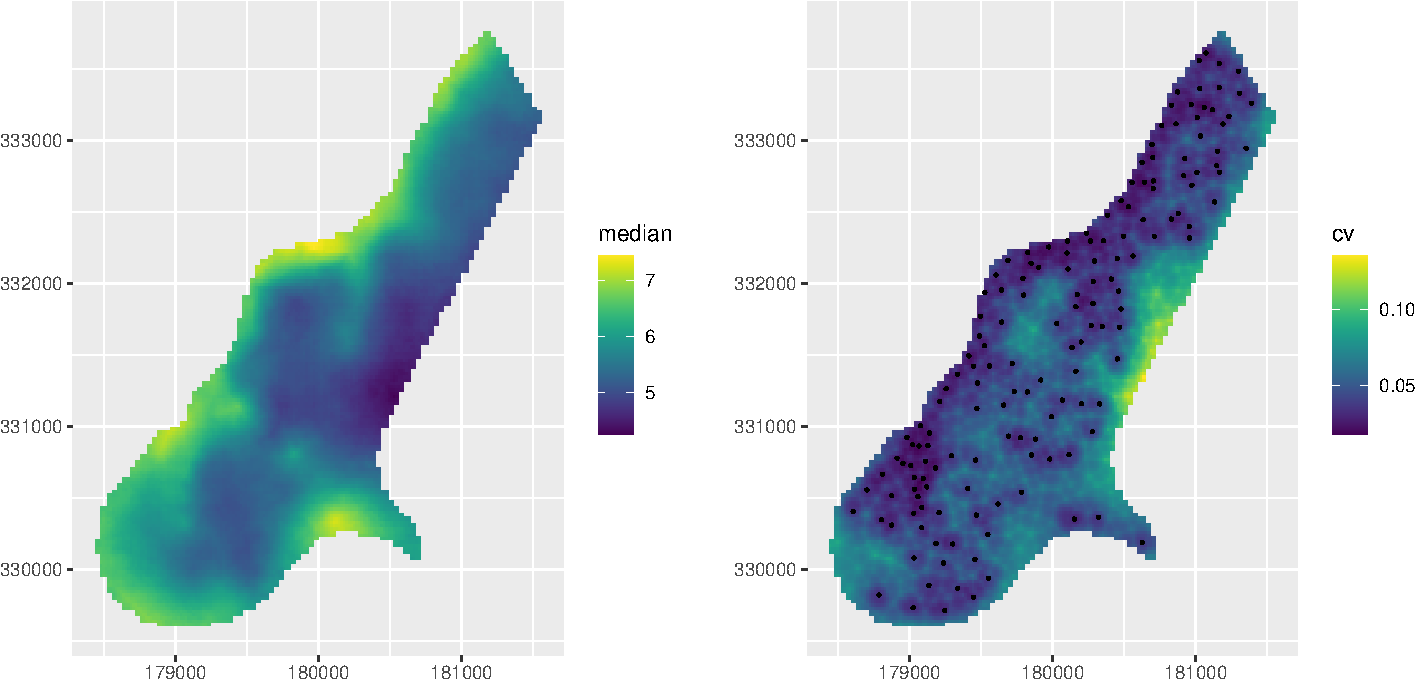
\includegraphics[width=0.6\linewidth]{Part1_intro_files/figure-beamer/unnamed-chunk-20-1} \end{center}

\textcolor{red}{If $\bf{y} \mid \bf{x}, \bf{\theta}$ is Gaussian "the approximation" is exact!}
\}
\end{frame}

\begin{frame}{What do we get \ldots{}}
\protect\hypertarget{what-do-we-get}{}
\[
\widetilde{\pi}(\bf{\theta} \mid \bf{y}) \propto  \frac{
           \pi(\bf{x}, \bf{y}\mid \bf{\theta})
        \; \pi(\bf{\theta})}{\widetilde{\pi}_G(\bf{x} \mid \bf{y},
            \bf{\theta})} \: \Bigg|_{\bf{x} = \bf{x}^\star(\bf{\theta})}
\]

\begin{itemize}
\item
  find the mode of \(\widetilde{\pi}(\bf{\theta}\mid \bf{y})\)
  (optimization)
\item
  explore \(\widetilde{\pi}(\bf{\theta}\mid \bf{y})\) to find grid
  points \(t_k\) for numerical integration.\\
  \strut \\
  \strut \\
\end{itemize}

\pause

However, why is it called \textcolor{red}{integrated nested Laplace
      approximation}?

\pause

There is another step that changes:

\[
\pi(x_{i} \mid \bf{y}) \approx \sum_k \underbrace{\pi(x_{i} \mid \bf{y}, \theta^k)}_{{\text{Not Gaussian!}}}{\widetilde{\pi}_G(\theta^k\mid\bf{y})} \Delta_k
\]
\end{frame}

\begin{frame}{Approximating \(\pi(x_i|\bf{y}, \bf{\theta})\)}
\protect\hypertarget{approximating-pix_ibfy-bftheta}{}
Three possible approximations:

\begin{itemize}[<+->]
\item
  \begin{enumerate}[<+->]
  \tightlist
  \item
    \textcolor{red}{Gaussian distribution} derived from
    \(\widetilde{\pi}_G(\bf{x}|\bf{\theta}, \bf{y})\), i.e. \[
    \widetilde{\pi}(x_i|\bf{\theta}, \bf{y}) = \mathcal{N}(x_i; \mu_i(\bf{\theta}), \sigma_i^2(\bf{\theta}))
    \] with mean \(\mu_i(\bf{\theta})\) and marginal variance
    \(\sigma_i^2(\bf{\theta})\).
  \end{enumerate}
\end{itemize}

However, errors in location and/or lack of skewness possible

\begin{itemize}[<+->]
\item
  \begin{enumerate}[<+->]
  \setcounter{enumi}{1}
  \tightlist
  \item
    \textcolor{red}{Laplace approximation}
  \end{enumerate}
\item
  \begin{enumerate}[<+->]
  \setcounter{enumi}{2}
  \tightlist
  \item
    \textcolor{red}{Simplified Laplace approximation}
  \end{enumerate}
\end{itemize}
\end{frame}

\begin{frame}[fragile]{Laplace approximation of
\(\pi(x_i|\bf{\theta}, \bf{y})\)}
\protect\hypertarget{laplace-approximation-of-pix_ibftheta-bfy}{}
\[
\widetilde{\pi}_\text{LA}(x_i|\bf{\theta}, \bf{y}) \propto
            \frac{\pi(\bf{x}, \bf{\theta},\bf{y})}
            {\widetilde{\pi}_\text{GG}(\bf{x}_{-i}|x_i, \bf{\theta}, \bf{y})}
            \Biggr|_{\bf{x}_{-i}=\bf{x^\star}_{-i}(x_i, \bf{\theta})}
\]

The approximation is very good but expensive as \(n\) factorizations of
\((n-1) \times (n-1)\) matrices are required to get the \(n\) marginals.

\pause

\textcolor{blue}{Computational modifications exist:}

\begin{enumerate}
\item
  Approximate the modal configuration of the GMRF approximation.
\item
\begin{verbatim}
 \item Reduce the size $n$ by only involving the ``neighbors''.
\end{verbatim}
\end{enumerate}
\end{frame}

\begin{frame}{Simplified Laplace approximation}
\protect\hypertarget{simplified-laplace-approximation}{}
Faster alternative to the Laplace approximation\\

\begin{itemize}
\tightlist
\item
  based on a \textcolor{red}{series
   expansion up to third order of the numerator and denominator of $\widetilde{\pi}_\text{LA}(x_i|\bf{\theta}, \bf{y})$}
\item
  corrects the Gaussian approximation for error in location and lack of
  skewness.
\end{itemize}

\pause

This is \textcolor{red}{default option when using INLA} but this choice
can be modified.
\end{frame}

\begin{frame}{INLA: Overview}
\protect\hypertarget{inla-overview}{}
\begin{itemize}
\item
  \textbf{Step I} Approximate \(\pi({\theta}|y)\) using the Laplace
  approximation and select good evaluation points \({\theta}_k\).
\item
  \textbf{Step II} For each \({\theta}_k\) and \(i\) approximate
  \(\pi(x_i|{\theta}_k, {y})\) using the Laplace or simplified Laplace
  approximation for selected values of \(x_i\)
\item
  \textbf{Step III} For each \(i\), sum out \({\theta}_k\)
  \[                
  \widetilde{\pi}(x_i|{y}) = \sum_k \widetilde{\pi}(x_i|{\theta}_k, {y}) \times
                    \widetilde{\pi}({\theta}_k|{y}) \times \Delta_k.
  \] Build a log spline corrected Gaussian to represent
  \(\widetilde{\pi}(x_i|{y})\).
\end{itemize}
\end{frame}

\begin{frame}{INLA: Why does it work?}
\protect\hypertarget{inla-why-does-it-work}{}
\begin{itemize}
\item
  The full conditional \(\pi(x|y,\theta)\) is ``almost'' Gaussian
\item
  The latent field \(x\) is a GMRF

  \begin{itemize}
  \tightlist
  \item
    GMRF \(\rightarrow\) sparse precision matrix!!
  \item
    Easy to solve and store
  \end{itemize}
\item
  Smart numerical methods
\item
  Parallel implementation
\end{itemize}
\end{frame}

\begin{frame}{Limitations}
\protect\hypertarget{limitations}{}
\begin{itemize}
\item
  The dimension of the latent field \(x\) can be large (\(10^2-10^6\))
\item
  The dimension of the hyperparameters \(\theta\) must be small
  (\(\leq 9\))
\end{itemize}

In other words, each random effect can be big, but there cannot be too
many random effects unless they share parameters.
\end{frame}

\begin{frame}{INLA features}
\protect\hypertarget{inla-features}{}
INLA fully incorporates posterior uncertainty with respect to
hyperparameters \(\Rightarrow\) tool for full Bayesian inference

\begin{itemize}
\tightlist
\item
  Marginal posterior densities of all (hyper-)parameters
\item
  Posterior mean, median, quantiles, std.\textasciitilde deviation, etc.
\item
  The approach can be used for predictions, model assessment, \ldots
\item
  Joint posterior marginal not available\ldots but it is possible to
  sample from \(\widetilde{\pi}(x,\theta|y)\)
\end{itemize}
\end{frame}

\begin{frame}{}
\protect\hypertarget{section-1}{}
\Large

Thank you for your attention!

\normalsize

If you have any doubts or questions, please write :
\url{sara.martino@math.ntnu.no}

\begin{center}
\includegraphics[width=0.3\linewidth]{graphics/smiley_small} \end{center}
\end{frame}

\end{document}
